% =====================================================================
%  RF Engineering Workbench — Guía de estudio personal (XeLaTeX)
%  Los valores numéricos de los ejemplos y las figuras se generan con el
%  motor de la aplicación: docs/src/guia_latex.py → generado/
% =====================================================================
\documentclass[11pt,a4paper,openany,oneside]{book}
\usepackage[a4paper,top=2.4cm,bottom=2.3cm,left=2.4cm,right=2.4cm,headheight=15pt]{geometry}
\usepackage{fontspec}
\usepackage{amsmath,amssymb,mathtools}
\usepackage{unicode-math}
\setmainfont{Cambria}
\setsansfont{Calibri}
\setmonofont{Consolas}[Scale=0.88]
\setmathfont{Cambria Math}
\usepackage{polyglossia}
\setdefaultlanguage{spanish}
\usepackage{siunitx}
\sisetup{output-decimal-marker={.},group-separator={\,},per-mode=symbol}
\DeclareSIUnit{\neper}{Np}\DeclareSIUnit{\dBi}{dBi}\DeclareSIUnit{\var}{var}\DeclareSIUnit{\dBm}{dBm}
\usepackage{graphicx,xcolor,booktabs,longtable,tabularx,array,enumitem,multicol,caption}
\usepackage[most]{tcolorbox}
\usepackage{tikz}
\usetikzlibrary{arrows.meta,positioning,calc,decorations.pathmorphing}
\usepackage{fancyhdr,titlesec}
\usepackage[hidelinks,bookmarksnumbered]{hyperref}

% ---------- colores ----------
\definecolor{acc}{HTML}{059669}\definecolor{accD}{HTML}{064E3B}\definecolor{accL}{HTML}{ECFDF5}
\definecolor{inf}{HTML}{2563EB}\definecolor{infL}{HTML}{EFF6FF}
\definecolor{wrn}{HTML}{D97706}\definecolor{wrnL}{HTML}{FFFBEB}
\definecolor{vio}{HTML}{7C3AED}\definecolor{vioL}{HTML}{F5F3FF}
\definecolor{gry}{HTML}{475569}\definecolor{gryL}{HTML}{F1F5F9}
\definecolor{band}{HTML}{0B1220}

% ---------- notación ----------
\newcommand{\jj}{\mathrm{j}}                 % unidad imaginaria (ingeniería)
\newcommand{\dd}{\mathrm{d}}                 % diferencial
\newcommand{\ee}{\mathrm{e}}                 % número e
\renewcommand{\Re}{\operatorname{Re}}
\renewcommand{\Im}{\operatorname{Im}}
\newcommand{\conj}[1]{#1^{*}}
\newcommand{\abs}[1]{\left|#1\right|}
\newcommand{\app}[1]{\textsf{\textbf{#1}}}  % nombre de módulo de la aplicación

% ---------- títulos ----------
\titleformat{\chapter}[display]{\sffamily\bfseries\color{accD}}{\large\color{acc}\MakeUppercase{\chaptertitlename}~\thechapter}{4pt}{\Huge}
\titlespacing*{\chapter}{0pt}{-10pt}{18pt}
\titleformat{\section}{\sffamily\bfseries\Large\color{accD}}{\thesection}{0.6em}{}
\titleformat{\subsection}{\sffamily\bfseries\large\color{black}}{\thesubsection}{0.6em}{}
\titleformat{\part}[display]{\centering\sffamily\bfseries\color{accD}}{\Large\color{acc}PARTE~\thepart}{10pt}{\Huge}
\renewcommand{\thepart}{\Roman{part}}

% ---------- cabeceras (sin nombre del autor en cada página) ----------
\pagestyle{fancy}\fancyhf{}
\fancyhead[L]{\small\sffamily\color{gry}RF Engineering Workbench — Guía de estudio}
\fancyhead[R]{\small\sffamily\color{gry}Versión \Version}
\fancyfoot[C]{\small\sffamily\thepage}
\renewcommand{\headrulewidth}{0.4pt}
\fancypagestyle{plain}{\fancyhf{}\fancyfoot[C]{\small\sffamily\thepage}\renewcommand{\headrulewidth}{0pt}}

% ---------- cuadros ----------
\tcbset{base/.style={enhanced,boxrule=0pt,leftrule=3pt,sharp corners,fonttitle=\sffamily\bfseries\small,
  before skip=8pt,after skip=10pt,left=8pt,right=8pt,top=5pt,bottom=6pt}}
\newtcolorbox{definicion}[1]{base,colback=accL,colframe=acc,colbacktitle=accL,coltitle=accD,title={Definición — #1}}
\newtcolorbox{ejemplo}[1]{base,colback=infL,colframe=inf,colbacktitle=infL,coltitle=inf,title={Ejemplo resuelto — #1}}
\newtcolorbox{intuicion}[1][]{base,colback=vioL,colframe=vio,colbacktitle=vioL,coltitle=vio,title={Intuición física#1}}
\newtcolorbox{atencion}[1]{base,colback=wrnL,colframe=wrn,colbacktitle=wrnL,coltitle=wrn!80!black,title={Atención — #1}}
\newtcolorbox{enlaapp}{base,colback=gryL,colframe=gry,colbacktitle=gryL,coltitle=gry,title={En la aplicación}}

% ---------- bloque «donde:» que explica cada símbolo ----------
\newenvironment{donde}{\par\vspace{2pt}\noindent{\small\itshape donde:}\par\noindent\small
  \tabularx{\linewidth}{@{\hspace{1.4em}}>{\raggedleft\arraybackslash}p{2.7cm}@{\hspace{0.9em}}X@{\hspace{0.6em}}>{\raggedleft\arraybackslash}p{2.3cm}@{}}}
  {\endtabularx\par\medskip}
\newcommand{\sym}[3]{$#1$ & #2 & \textcolor{gry}{#3}\\[1pt]}

\setlist{itemsep=2pt,topsep=4pt}
\captionsetup{font={small,sf},labelfont=bf}
\renewcommand{\arraystretch}{1.18}
\numberwithin{equation}{chapter}
\makeatletter\renewcommand\@endpart{\vfil\newpage}\makeatother % sin página en blanco tras cada parte

\makeatletter\newcommand{\tabla}[1]{\@@input #1 }\makeatother % \input expandible dentro de tablas
\input{generado/valores}

\begin{document}
\frontmatter
% ---------------------------- portada ----------------------------
\begin{titlepage}
\begin{tikzpicture}[remember picture,overlay]
  \fill[band] (current page.north west) rectangle ([yshift=-0.6\paperheight]current page.north east);
  \begin{scope}[shift={([xshift=-5.2cm,yshift=-6cm]current page.north east)},line width=1.6pt,color=acc!70!white]
    \draw (0,0) circle (3.2);
    \foreach \r in {0.5,1,3}{\pgfmathsetmacro{\rr}{3.2/(1+\r)}\draw[line width=0.6pt] ({3.2-\rr},0) circle (\rr);}
    \draw[line width=0.6pt] (-3.2,0) -- (3.2,0);
  \end{scope}
  \node[anchor=north west,text=acc!70!white,font=\ttfamily\small] at ([xshift=2.2cm,yshift=-2.2cm]current page.north west) {GUÍA DE ESTUDIO PERSONAL};
  \node[anchor=south west,text width=15cm,text=white,font=\sffamily\bfseries\fontsize{30}{36}\selectfont] at ([xshift=2.2cm,yshift=-15.2cm]current page.north west) {RF Engineering\\ Workbench};
  \node[anchor=north west,text width=15.5cm,text=acc!45!white,font=\sffamily\Large] at ([xshift=2.2cm,yshift=-15.6cm]current page.north west)
     {De los principios matemáticos al funcionamiento: un repaso profundo de la teoría de RF que implementa la aplicación};
  \node[anchor=north west,text width=16cm,font=\sffamily\large,text=black] at ([xshift=2.2cm,yshift=-19.8cm]current page.north west)
     {\textbf{Ricardo Villalobos Perez}\\[2pt]{\normalsize\color{gry}Versión de la aplicación \Version}};
  \node[anchor=north west,text width=16cm,font=\small,text=gry] at ([xshift=2.2cm,yshift=-22.3cm]current page.north west)
     {Todas las fórmulas de este documento son las que usa el motor de la aplicación. Los valores numéricos de los ejemplos
      y las figuras se han calculado con ese mismo motor al generar el documento.};
\end{tikzpicture}
\end{titlepage}

\tableofcontents
\chapter*{Cómo usar esta guía}
\addcontentsline{toc}{chapter}{Cómo usar esta guía}

Esta guía es un repaso profundo, ordenado de lo más básico a lo más avanzado. Cada capítulo se apoya en los anteriores, así que
conviene leerla en orden la primera vez. Después puede usarse como consulta.

\begin{itemize}
  \item La \textbf{Parte I} construye las herramientas matemáticas: números complejos, fasores, impedancia, potencia,
        resonancia y decibelios.
  \item La \textbf{Parte II} desarrolla la teoría de radiofrecuencia exactamente como la implementa el motor: líneas,
        reflexión, carta de Smith, adaptación, parámetros S, estabilidad, modo mixto, dominio del tiempo, calibración, antenas y microstrip.
  \item La \textbf{Parte III} explica cómo está construida la aplicación, cómo se usa cada módulo y cómo se mantiene y publica.
\end{itemize}

Cada ecuación importante va seguida de un bloque \emph{«donde:»} que explica qué significa cada símbolo y en qué unidades se mide.
Los cuadros tienen un significado fijo:

\begin{definicion}{qué es}Definiciones formales de los conceptos.\end{definicion}
\begin{intuicion}[: qué significa]Explicación del concepto sin fórmulas: qué ocurre físicamente y por qué importa.\end{intuicion}
\begin{ejemplo}{con números}Ejercicios resueltos paso a paso. Los valores los ha calculado el motor de la aplicación.\end{ejemplo}
\begin{atencion}{errores frecuentes}Convenciones, trampas y confusiones habituales.\end{atencion}
\begin{enlaapp}Dónde aparece el concepto en la aplicación y cómo usarlo.\end{enlaapp}

% =====================================================================
\chapter*{Nomenclatura}
\addcontentsline{toc}{chapter}{Nomenclatura}

\section*{Matemática general}
\begin{longtable}{@{}>{\centering\arraybackslash}p{2.6cm}p{9.6cm}p{2.4cm}@{}}
\toprule \textbf{Símbolo} & \textbf{Significado} & \textbf{Unidad}\\ \midrule\endhead
$\jj$ & Unidad imaginaria, $\jj^2=-1$ (en ingeniería no se usa $i$ para no confundirla con la corriente) & --- \\
$z = a + \jj b$ & Número complejo genérico: $a$ parte real, $b$ parte imaginaria & --- \\
$\abs{z}$, $\varphi$ & Módulo (longitud) y argumento (ángulo) de un número complejo & ---, rad o $^\circ$ \\
$\conj{z}$ & Conjugado: cambia el signo de la parte imaginaria & --- \\
$\Re\{\cdot\}$, $\Im\{\cdot\}$ & Parte real y parte imaginaria & --- \\
$\ee^{\jj\varphi}$ & Exponencial compleja (fórmula de Euler) & --- \\
$\angle$ & «con ángulo»: $10\angle 30^\circ$ es un número de módulo 10 y ángulo $30^\circ$ & --- \\
$\ln$, $\log_{10}$ & Logaritmo natural (base $\ee$) y decimal & --- \\
$\mathcal{F}$, $\mathcal{F}^{-1}$ & Transformada de Fourier y su inversa & --- \\
\bottomrule
\end{longtable}

\section*{Señales y circuitos}
\begin{longtable}{@{}>{\centering\arraybackslash}p{2.6cm}p{9.6cm}p{2.4cm}@{}}
\toprule \textbf{Símbolo} & \textbf{Significado} & \textbf{Unidad}\\ \midrule\endhead
$t$ & Tiempo & \si{\second} \\
$f$ & Frecuencia: número de oscilaciones por segundo & \si{\hertz} \\
$\omega = 2\pi f$ & Frecuencia angular: radianes recorridos por segundo & \si{\radian\per\second} \\
$T = 1/f$ & Periodo: duración de una oscilación & \si{\second} \\
$v(t)$, $i(t)$ & Tensión y corriente instantáneas (valores reales en el tiempo) & \si{\volt}, \si{\ampere} \\
$V$, $I$ & Fasores de tensión y corriente (números complejos) & \si{\volt}, \si{\ampere} \\
$R$ & Resistencia: se opone a la corriente disipando energía & \si{\ohm} \\
$L$ & Inductancia: almacena energía en el campo magnético & \si{\henry} \\
$C$ & Capacidad: almacena energía en el campo eléctrico & \si{\farad} \\
$Z = R + \jj X$ & Impedancia: oposición compleja al paso de corriente alterna & \si{\ohm} \\
$X$ & Reactancia: parte imaginaria de $Z$ (positiva inductiva, negativa capacitiva) & \si{\ohm} \\
$X_L$, $X_C$ & Reactancia de una bobina y de un condensador & \si{\ohm} \\
$Y = G + \jj B$ & Admitancia, inversa de la impedancia & \si{\siemens} \\
$G$, $B$ & Conductancia y susceptancia & \si{\siemens} \\
$S = P + \jj Q$ & Potencia compleja & \si{\volt\ampere} \\
$P$ & Potencia activa (la que realmente se consume o transmite) & \si{\watt} \\
$Q$ & Potencia reactiva (energía que va y vuelve) — no confundir con el factor de calidad & var \\
$f_0$ & Frecuencia de resonancia & \si{\hertz} \\
$Q$ (factor) & Factor de calidad: relación entre energía almacenada y disipada por ciclo & --- \\
$BW$ & Ancho de banda & \si{\hertz} \\
\bottomrule
\end{longtable}

\section*{Líneas de transmisión y ondas}
\begin{longtable}{@{}>{\centering\arraybackslash}p{2.6cm}p{9.6cm}p{2.4cm}@{}}
\toprule \textbf{Símbolo} & \textbf{Significado} & \textbf{Unidad}\\ \midrule\endhead
$c$ & Velocidad de la luz en el vacío, $\num{299792458}$ & \si{\metre\per\second} \\
$\lambda$, $\lambda_0$ & Longitud de onda en la línea y en el vacío & \si{\metre} \\
$v_p$ & Velocidad de fase de la onda en la línea & \si{\metre\per\second} \\
$v_f = v_p/c$ & Factor de velocidad & --- \\
$\varepsilon_r$, $\varepsilon_{\text{eff}}$ & Permitividad relativa del dieléctrico y efectiva (microstrip) & --- \\
$R', L', G', C'$ & Parámetros distribuidos: resistencia, inductancia, conductancia y capacidad \emph{por metro} & \si{\ohm\per\metre}, \si{\henry\per\metre}, \si{\siemens\per\metre}, \si{\farad\per\metre} \\
$Z_0$ & Impedancia característica de la línea (o impedancia de referencia) & \si{\ohm} \\
$\gamma = \alpha + \jj\beta$ & Constante de propagación & \si{\per\metre} \\
$\alpha$ & Constante de atenuación & \si{\neper\per\metre} \\
$\beta = 2\pi/\lambda$ & Constante de fase (número de onda) & \si{\radian\per\metre} \\
$\ell$ & Longitud física de la línea & \si{\metre} \\
$d$ & Distancia medida desde la carga hacia el generador & \si{\metre} \\
$\theta = \beta\ell$ & Longitud eléctrica & \si{\radian} o $^\circ$ \\
$V^+$, $V^-$ & Amplitudes de la onda incidente y de la reflejada & \si{\volt} \\
$Z_L$, $Z_{in}$ & Impedancia de carga y de entrada & \si{\ohm} \\
$\delta_s$ & Profundidad de penetración (efecto pelicular) & \si{\metre} \\
$R_s$ & Resistencia superficial del conductor & \si{\ohm} \\
\bottomrule
\end{longtable}

\section*{Reflexión, adaptación y redes}
\begin{longtable}{@{}>{\centering\arraybackslash}p{2.6cm}p{9.6cm}p{2.4cm}@{}}
\toprule \textbf{Símbolo} & \textbf{Significado} & \textbf{Unidad}\\ \midrule\endhead
$\Gamma$ & Coeficiente de reflexión (complejo) & --- \\
$\Gamma_L$, $\Gamma_{in}$ & Coeficiente de reflexión en la carga y en la entrada & --- \\
$z = Z/Z_0 = r + \jj x$ & Impedancia normalizada (sin unidades) & --- \\
$y = 1/z = g + \jj b$ & Admitancia normalizada & --- \\
$\mathrm{VSWR}$ (ROE) & Relación de onda estacionaria & --- \\
$RL$ & Return Loss, pérdida de retorno (positiva) & \si{\decibel} \\
$ML$ & Mismatch loss, pérdida por desadaptación & \si{\decibel} \\
$Z_s$ & Impedancia de la fuente & \si{\ohm} \\
$\Gamma_p$ & Coeficiente de reflexión de onda de potencia (para fuentes complejas) & --- \\
$Q_L$ & Factor de calidad de la carga, $\abs{X_L}/R_L$ & --- \\
$\Gamma_m$ & Máxima reflexión admitida en la banda de adaptación & --- \\
$G_T$ & Ganancia de transductor & --- o \si{\decibel} \\
$A, B, C, D$ & Parámetros de la matriz de transmisión (cascada) & mixtas \\
\bottomrule
\end{longtable}

\section*{Parámetros S, estabilidad y antenas}
\begin{longtable}{@{}>{\centering\arraybackslash}p{2.6cm}p{9.6cm}p{2.4cm}@{}}
\toprule \textbf{Símbolo} & \textbf{Significado} & \textbf{Unidad}\\ \midrule\endhead
$a_i$, $b_i$ & Ondas de potencia incidente y reflejada en el puerto $i$ & $\sqrt{\mathrm{W}}$ \\
$S_{ij}$ & Parámetro S: respuesta en el puerto $i$ a una excitación en el puerto $j$ & --- \\
$\Delta$ & Determinante de la matriz S de dos puertos & --- \\
$K$, $\mu$ & Factores de estabilidad de Rollett y de Edwards–Sinsky & --- \\
$\tau_g$ & Retardo de grupo & \si{\second} \\
$S_{dd}$, $S_{cc}$, $S_{dc}$ & Parámetros en modo mixto: diferencial, común y conversión & --- \\
$e_{00}$, $e_{11}$, $e_{10}e_{01}$ & Términos de error de la calibración de un puerto & --- \\
$\eta_0$ & Impedancia del espacio libre, $\approx \SI{376.73}{\ohm}$ & \si{\ohm} \\
$k = 2\pi/\lambda$ & Número de onda en el espacio libre & \si{\radian\per\metre} \\
$F(\theta)$ & Diagrama de campo (dependencia angular) & --- \\
$R_r$, $R_L$ & Resistencia de radiación y de pérdidas de la antena & \si{\ohm} \\
$D$, $G$, $e$ & Directividad, ganancia y eficiencia de radiación & ---, \si{\dBi} \\
$\sigma$, $\mu_0$ & Conductividad del metal y permeabilidad del vacío ($4\pi\times10^{-7}$) & \si{\siemens\per\metre}, \si{\henry\per\metre} \\
\bottomrule
\end{longtable}

\section*{Prefijos del Sistema Internacional}
La aplicación acepta estos prefijos al escribir valores: \texttt{10n} = \SI{10}{\nano\henry} si es una bobina, \texttt{4.7p} = \SI{4.7}{\pico\farad}, \texttt{433MHz}, \texttt{2.4G}.
\begin{center}
\begin{tabular}{cccccccccc}\toprule
f & p & n & µ (u) & m & --- & k & M & G & T\\\midrule
$10^{-15}$ & $10^{-12}$ & $10^{-9}$ & $10^{-6}$ & $10^{-3}$ & $1$ & $10^{3}$ & $10^{6}$ & $10^{9}$ & $10^{12}$\\\bottomrule
\end{tabular}
\end{center}


\mainmatter
\part{Fundamentos matemáticos}
\chapter{Números complejos}

Casi todo en radiofrecuencia se calcula con números complejos. No es un artificio: una señal alterna tiene \emph{amplitud} y \emph{fase},
y un número complejo guarda exactamente esas dos informaciones en un solo objeto. Este capítulo construye todo lo necesario desde cero.

\section{Qué es un número complejo}

\begin{definicion}{número complejo}
Un número complejo es un par ordenado de números reales que se escribe
\begin{equation}
  z = a + \jj\,b, \qquad \jj^2 = -1 .
\end{equation}
\begin{donde}
\sym{z}{el número complejo}{---}
\sym{a = \Re\{z\}}{\textbf{parte real}: la componente horizontal}{---}
\sym{b = \Im\{z\}}{\textbf{parte imaginaria}: la componente vertical (es un número real)}{---}
\sym{\jj}{unidad imaginaria; en electricidad se escribe $\jj$ porque $i$ se reserva para la corriente}{---}
\end{donde}
\end{definicion}

Un número complejo se dibuja como un \textbf{punto} (o una flecha desde el origen) en el \emph{plano complejo}: el eje horizontal es la parte real y el vertical la imaginaria.

\begin{center}
\begin{tikzpicture}[scale=1.15,>=Stealth]
  \draw[->,gry] (-0.6,0) -- (4.4,0) node[right,black] {$\Re$};
  \draw[->,gry] (0,-0.6) -- (0,3.0) node[above,black] {$\Im$};
  \draw[->,very thick,acc] (0,0) -- (3.4,2.2) node[above right,black] {$z=a+\jj b$};
  \draw[dashed,gry] (3.4,0) -- (3.4,2.2) (0,2.2) -- (3.4,2.2);
  \node[below] at (3.4,0) {$a$}; \node[left] at (0,2.2) {$b$};
  \draw[->,inf] (1.1,0) arc (0:32.9:1.1); \node[inf] at (1.45,0.35) {$\varphi$};
  \node[acc,rotate=33] at (1.55,1.3) {$\abs{z}$};
  \fill[wrn] (3.4,-2.2) circle (2pt) node[right,black] {$\conj z = a-\jj b$};
  \draw[dashed,wrn] (3.4,-0.05) -- (3.4,-2.1);
\end{tikzpicture}
\end{center}

\section{Forma polar: módulo y argumento}

La misma flecha puede describirse por su \textbf{longitud} y su \textbf{ángulo}. Por el teorema de Pitágoras y la trigonometría:
\begin{equation}
  \abs{z} = \sqrt{a^2 + b^2}, \qquad \varphi = \operatorname{atan2}(b,\,a), \qquad a = \abs{z}\cos\varphi, \quad b = \abs{z}\sin\varphi .
\end{equation}
\begin{donde}
\sym{\abs{z}}{\textbf{módulo}: distancia del punto al origen (siempre $\geq 0$)}{---}
\sym{\varphi}{\textbf{argumento} o fase: ángulo medido desde el eje real positivo, en sentido antihorario}{rad o $^\circ$}
\sym{\operatorname{atan2}(b,a)}{arcotangente de $b/a$ que tiene en cuenta el cuadrante (signos de $a$ y $b$)}{rad}
\end{donde}

\begin{atencion}{atan2 y no arctan}
$\arctan(b/a)$ no distingue $z = 1+\jj$ (ángulo $45^\circ$) de $z = -1-\jj$ (ángulo $-135^\circ$), porque ambos dan $b/a = 1$.
La función $\operatorname{atan2}$ mira los signos de $a$ y $b$ por separado y devuelve el ángulo correcto entre $-180^\circ$ y $180^\circ$.
La aplicación usa siempre $\operatorname{atan2}$.
\end{atencion}

\section{La fórmula de Euler}

La herramienta clave que une exponenciales y trigonometría es la fórmula de Euler:
\begin{equation}
  \ee^{\jj\varphi} = \cos\varphi + \jj\,\sin\varphi .
\end{equation}
\begin{donde}
\sym{\ee}{número de Euler, $\approx 2.71828$, base de los logaritmos naturales}{---}
\sym{\varphi}{ángulo}{rad}
\end{donde}
Gracias a ella, todo número complejo se escribe en \textbf{forma exponencial}:
\begin{equation}
  z = \abs{z}\,\ee^{\jj\varphi} = \abs{z}\angle\varphi .
\end{equation}

\begin{intuicion}[: multiplicar por $\ee^{\jj\varphi}$ es girar]
$\ee^{\jj\varphi}$ es un número de módulo 1 y ángulo $\varphi$: un punto sobre la circunferencia unidad. Multiplicar cualquier número
por $\ee^{\jj\varphi}$ \emph{no cambia su tamaño, sólo lo gira} un ángulo $\varphi$. Esta idea reaparece constantemente: una señal
que oscila en el tiempo es una flecha que gira ($\ee^{\jj\omega t}$), y una onda que avanza por una línea hace girar el coeficiente
de reflexión sobre la carta de Smith ($\ee^{-\jj2\beta d}$).
\end{intuicion}

\section{Operaciones}

\begin{itemize}
\item \textbf{Suma y resta}: se suman las partes reales y las imaginarias por separado (como vectores). Es cómodo en forma rectangular:
\begin{equation}
  (a_1 + \jj b_1) + (a_2 + \jj b_2) = (a_1 + a_2) + \jj(b_1 + b_2).
\end{equation}
\item \textbf{Producto}: en forma polar se multiplican los módulos y se \emph{suman} los ángulos:
\begin{equation}
  z_1 z_2 = \abs{z_1}\abs{z_2}\,\ee^{\jj(\varphi_1 + \varphi_2)} .
\end{equation}
\item \textbf{Cociente}: se dividen los módulos y se \emph{restan} los ángulos. En forma rectangular se multiplica arriba y abajo por el conjugado del denominador:
\begin{equation}
  \frac{z_1}{z_2} = \frac{z_1\,\conj{z_2}}{z_2\,\conj{z_2}} = \frac{z_1\,\conj{z_2}}{\abs{z_2}^2} .
\end{equation}
\end{itemize}

\begin{definicion}{conjugado}
\begin{equation}
  \conj{z} = a - \jj b = \abs{z}\,\ee^{-\jj\varphi}, \qquad z\,\conj{z} = a^2 + b^2 = \abs{z}^2 .
\end{equation}
El conjugado es la imagen especular respecto al eje real. Su propiedad más útil es que $z\conj{z}$ es siempre real y positivo:
por eso aparece al calcular potencias y en la condición de máxima transferencia de potencia ($Z_{\text{carga}} = \conj{Z_{\text{fuente}}}$).
\end{definicion}

\begin{ejemplo}{$z = 80 + \jj 30$}
\begin{align*}
  \abs{z} &= \sqrt{80^2 + 30^2} = \sqrt{7300} = \ZejMod \\
  \varphi &= \operatorname{atan2}(30, 80) = \ZejArg^\circ \\
  \frac{1}{z} &= \frac{\conj z}{\abs{z}^2} = \frac{80 - \jj30}{7300} = \ZejInv
\end{align*}
El inverso de una impedancia es la admitancia: este cálculo es exactamente el que hace la aplicación para obtener $Y = 1/Z$.
\end{ejemplo}

\begin{enlaapp}
La aplicación entiende varias notaciones al escribir impedancias: \texttt{80+j30}, \texttt{80 - j30 Ω}, \texttt{j25}, \texttt{-j10},
\texttt{30-12j} y la forma polar \texttt{100}$\angle$\texttt{45} (módulo y ángulo en grados). Internamente todo se convierte a un número complejo de Python.
\end{enlaapp}

\chapter{Señales senoidales, fasores e impedancia}

\section{La señal senoidal}

En régimen permanente, todas las tensiones y corrientes de un circuito lineal excitado por una fuente senoidal son senoides
de la \emph{misma frecuencia}; sólo cambian su amplitud y su fase. Una tensión senoidal se escribe:
\begin{equation}
  v(t) = V_p \cos(\omega t + \varphi), \qquad \omega = 2\pi f = \frac{2\pi}{T}.
\end{equation}
\begin{donde}
\sym{v(t)}{valor instantáneo de la tensión en el instante $t$}{\si{\volt}}
\sym{V_p}{amplitud de pico (valor máximo)}{\si{\volt}}
\sym{\omega}{frecuencia angular}{\si{\radian\per\second}}
\sym{f}{frecuencia}{\si{\hertz}}
\sym{T}{periodo}{\si{\second}}
\sym{\varphi}{fase inicial: desplazamiento de la onda respecto a un coseno que empieza en su máximo}{rad}
\end{donde}

\begin{definicion}{valor eficaz (RMS)}
El valor eficaz es el valor de una tensión continua que disiparía la misma potencia media en una resistencia.
Para una senoide:
\begin{equation}
  V_{\text{ef}} = \frac{V_p}{\sqrt{2}} \approx 0.707\,V_p .
\end{equation}
Las potencias se calculan con valores eficaces. La aplicación usa valores eficaces en el cálculo de potencias del \app{Impedance Analyzer}.
\end{definicion}

\section{El fasor}

\begin{definicion}{fasor}
El fasor de $v(t)$ es el número complejo que guarda su amplitud y su fase:
\begin{equation}
  V = V_p\,\ee^{\jj\varphi} \qquad\text{de modo que}\qquad v(t) = \Re\{V\,\ee^{\jj\omega t}\} .
\end{equation}
\begin{donde}
\sym{V}{fasor (número complejo): módulo $=$ amplitud, argumento $=$ fase}{\si{\volt}}
\sym{\ee^{\jj\omega t}}{factor de giro: una flecha de módulo 1 que gira a $\omega$ radianes por segundo}{---}
\sym{\Re\{\cdot\}}{parte real: la proyección de la flecha giratoria sobre el eje horizontal}{---}
\end{donde}
\end{definicion}

\begin{intuicion}[: la flecha que gira]
Imagine una flecha de longitud $V_p$ que gira en el plano complejo a velocidad constante $\omega$. Su sombra sobre el eje horizontal
sube y baja describiendo exactamente $V_p\cos(\omega t + \varphi)$. Como todas las señales del circuito giran a la misma
velocidad, podemos «congelar» el giro y trabajar sólo con la posición inicial de cada flecha: eso es el fasor.
\end{intuicion}

\subsection{\texorpdfstring{Por qué derivar es multiplicar por $\jj\omega$}{Por qué derivar es multiplicar por jω}}
Derivemos $\Re\{V\ee^{\jj\omega t}\}$ respecto al tiempo. Como $V$ es constante:
\begin{equation}
  \frac{\dd}{\dd t}\Re\{V\ee^{\jj\omega t}\} = \Re\left\{V\,\frac{\dd}{\dd t}\ee^{\jj\omega t}\right\} = \Re\{(\jj\omega V)\,\ee^{\jj\omega t}\}.
\end{equation}
Es decir: \textbf{el fasor de la derivada es $\jj\omega$ por el fasor}. Las ecuaciones diferenciales de los circuitos
se convierten así en ecuaciones algebraicas con números complejos, que son mucho más fáciles de resolver.

\begin{atencion}{la convención de signo $\ee^{+\jj\omega t}$}
La aplicación (y la ingeniería eléctrica en general) usa $\ee^{+\jj\omega t}$. Algunos libros de física usan $\ee^{-\jj\omega t}$ y
escriben $-\jj$ donde nosotros escribimos $+\jj$. Con nuestra convención \textbf{la reactancia de una bobina es positiva y la de un
condensador negativa}. Al comparar resultados con otro libro o programa, compruebe siempre la convención.
\end{atencion}

\section{Impedancia de los elementos básicos}

\begin{definicion}{impedancia}
La impedancia es el cociente entre el fasor de tensión y el fasor de corriente de un elemento (ley de Ohm generalizada):
\begin{equation}
  Z = \frac{V}{I} = R + \jj X .
\end{equation}
\begin{donde}
\sym{Z}{impedancia (compleja)}{\si{\ohm}}
\sym{R = \Re\{Z\}}{resistencia: parte que \emph{disipa} energía (la convierte en calor o radiación)}{\si{\ohm}}
\sym{X = \Im\{Z\}}{reactancia: parte que \emph{almacena} energía y la devuelve cada ciclo}{\si{\ohm}}
\end{donde}
\end{definicion}

\paragraph{Resistencia.} La ley de Ohm $v = R\,i$ no tiene derivadas, así que $V = R\,I$ y
\begin{equation} Z_R = R . \end{equation}

\paragraph{Bobina.} La tensión en una bobina es proporcional a la variación de su corriente, $v = L\,\dd i/\dd t$. En fasores,
derivar es multiplicar por $\jj\omega$:
\begin{equation}
  V = L\,(\jj\omega I) \quad\Rightarrow\quad Z_L = \jj\omega L, \qquad X_L = \omega L > 0 .
\end{equation}
\begin{donde}
\sym{L}{inductancia}{\si{\henry}}
\sym{X_L}{reactancia inductiva: crece linealmente con la frecuencia}{\si{\ohm}}
\end{donde}

\paragraph{Condensador.} La corriente en un condensador es proporcional a la variación de su tensión, $i = C\,\dd v/\dd t$:
\begin{equation}
  I = C\,(\jj\omega V) \quad\Rightarrow\quad Z_C = \frac{1}{\jj\omega C} = -\,\frac{\jj}{\omega C}, \qquad X_C = -\frac{1}{\omega C} < 0 .
\end{equation}
\begin{donde}
\sym{C}{capacidad}{\si{\farad}}
\sym{X_C}{reactancia capacitiva: negativa, y su valor absoluto disminuye con la frecuencia}{\si{\ohm}}
\end{donde}
Para pasar de $1/\jj$ a $-\jj$ basta multiplicar arriba y abajo por $\jj$: $\frac{1}{\jj} = \frac{\jj}{\jj^2} = -\jj$.

\begin{intuicion}[: qué significan los signos]
En una bobina la corriente va \emph{retrasada} $90^\circ$ respecto a la tensión (la bobina «se resiste» a los cambios de corriente);
en un condensador va \emph{adelantada} $90^\circ$. El signo de la reactancia indica cuál de los dos comportamientos domina.
A frecuencias altas la bobina se parece a un circuito abierto ($X_L\to\infty$) y el condensador a un cortocircuito ($X_C\to 0$);
a frecuencias bajas, al revés. Este simple hecho explica casi todos los filtros y redes de adaptación.
\end{intuicion}

\section{Admitancia}

\begin{definicion}{admitancia}
\begin{equation}
  Y = \frac{1}{Z} = G + \jj B = \frac{R}{R^2+X^2} - \jj\,\frac{X}{R^2+X^2}.
\end{equation}
\begin{donde}
\sym{Y}{admitancia: facilidad con que circula la corriente}{\si{\siemens}}
\sym{G = \Re\{Y\}}{conductancia}{\si{\siemens}}
\sym{B = \Im\{Y\}}{susceptancia: $B>0$ capacitiva, $B<0$ inductiva (signos opuestos a la reactancia)}{\si{\siemens}}
\end{donde}
\end{definicion}
\begin{atencion}{$G$ no es $1/R$}
Salvo que $X = 0$, la conductancia \emph{no} es el inverso de la resistencia: $G = R/(R^2+X^2)$. Es un error muy frecuente.
\end{atencion}

\section{Asociación de impedancias}

Las reglas son las mismas que para resistencias, pero con números complejos:
\begin{equation}
  Z_{\text{serie}} = Z_1 + Z_2 + \cdots + Z_n , \qquad\qquad Y_{\text{paralelo}} = Y_1 + Y_2 + \cdots + Y_n .
\end{equation}
En serie circula la misma corriente y se suman las tensiones (por eso se suman impedancias); en paralelo hay la misma tensión y
se suman las corrientes (por eso se suman admitancias). Para dos elementos en paralelo:
\begin{equation}
  Z_1 \parallel Z_2 = \frac{Z_1 Z_2}{Z_1 + Z_2}.
\end{equation}

\begin{ejemplo}{RLC serie a \SI{100}{\mega\hertz}}
Con $R = \SI{10}{\ohm}$, $L = \SI{100}{\nano\henry}$ y $C = \SI{25}{\pico\farad}$:
\begin{align*}
  \omega &= 2\pi\cdot 10^{8} = \RlcW~\si{\radian\per\second}\\
  X_L &= \omega L = \RlcXl~\si{\ohm} \\
  X_C &= -\frac{1}{\omega C} = \RlcXc~\si{\ohm}\\
  Z &= R + \jj(X_L + X_C) = \RlcZ~\si{\ohm}\\
  \abs{Z} &= \RlcZmag~\si{\ohm}, \qquad \varphi = \RlcZdeg^\circ \quad(\text{ligeramente capacitivo})\\
  Y &= 1/Z = \RlcY~\si{\siemens}
\end{align*}
Las dos reactancias casi se anulan: estamos muy cerca de la resonancia (capítulo siguiente).
\end{ejemplo}

\begin{enlaapp}
El \app{Impedance Analyzer} calcula estas magnitudes para once topologías (R, L, C, RL, RC, LC y RLC en serie y en paralelo) y
muestra el desarrollo paso a paso. En el modo «Red personalizada» se escribe cualquier combinación, por ejemplo
\texttt{R(50) + (L(10n) || C(4.7p))}, donde \texttt{+} es serie y \texttt{||} es paralelo; el motor la reduce recursivamente con las reglas anteriores.
\end{enlaapp}

\chapter{Potencia, resonancia y decibelios}

\section{Potencia en corriente alterna}

En un circuito de alterna la potencia instantánea $p(t) = v(t)\,i(t)$ oscila. Lo que interesa es su \emph{valor medio}
(la energía que realmente se entrega por unidad de tiempo) y la energía que va y vuelve sin consumirse.

\begin{definicion}{potencia compleja}
Con fasores eficaces $V$ e $I$:
\begin{equation}
  S = V\,\conj{I} = P + \jj Q, \qquad P = \abs{V}\abs{I}\cos\varphi, \qquad Q = \abs{V}\abs{I}\sin\varphi .
\end{equation}
\begin{donde}
\sym{S}{potencia compleja; su módulo $\abs{S}$ es la potencia aparente}{\si{\volt\ampere}}
\sym{\conj{I}}{conjugado del fasor de corriente}{\si{\ampere}}
\sym{P}{potencia activa: la media de $p(t)$, la que se convierte en calor, radiación o trabajo}{\si{\watt}}
\sym{Q}{potencia reactiva: energía que se intercambia cada ciclo con bobinas y condensadores}{\si{\var}}
\sym{\varphi}{ángulo de la impedancia: desfase entre tensión y corriente}{rad}
\sym{\cos\varphi}{factor de potencia (FP)}{---}
\end{donde}
\end{definicion}

\paragraph{Por qué aparece el conjugado.} Si $V = \abs{V}\ee^{\jj\varphi_v}$ e $I = \abs{I}\ee^{\jj\varphi_i}$, entonces
$V\conj{I} = \abs{V}\abs{I}\ee^{\jj(\varphi_v - \varphi_i)}$: el conjugado hace que se \emph{resten} las fases, y lo que importa
para la potencia es precisamente el desfase entre tensión y corriente, no la fase absoluta de cada una.

Usando $V = Z I$ se obtienen las formas más útiles:
\begin{equation}
  S = Z\,\abs{I}^2 \quad\Rightarrow\quad P = R\,\abs{I}^2, \qquad Q = X\,\abs{I}^2 .
\end{equation}
Es decir: \textbf{sólo la resistencia consume potencia}; la reactancia sólo la hace oscilar.

\begin{atencion}{pico frente a eficaz}
Si se usan amplitudes de pico en lugar de eficaces, $S = \tfrac12 V_p\conj{I_p}$. El factor $\tfrac12$ es una fuente clásica de
errores de \SI{3}{\decibel}. La aplicación trabaja con valores eficaces.
\end{atencion}

\section{Máxima transferencia de potencia}

Una fuente con impedancia interna $Z_s = R_s + \jj X_s$ y tensión $V_s$ alimenta una carga $Z_L = R_L + \jj X_L$. La potencia en la carga es
\begin{equation}
  P_L = \frac{\abs{V_s}^2\,R_L}{(R_s + R_L)^2 + (X_s + X_L)^2}.
\end{equation}
Para maximizarla, primero se anula el término reactivo del denominador ($X_L = -X_s$) y después se deriva respecto a $R_L$,
obteniendo $R_L = R_s$. Juntas:
\begin{equation}
  Z_L = \conj{Z_s} \qquad\Rightarrow\qquad P_{\max} = P_{\text{disp}} = \frac{\abs{V_s}^2}{4R_s}.
\end{equation}
\begin{donde}
\sym{Z_s}{impedancia interna de la fuente}{\si{\ohm}}
\sym{Z_L}{impedancia de carga}{\si{\ohm}}
\sym{P_{\text{disp}}}{potencia disponible: la máxima que puede entregar la fuente}{\si{\watt}}
\end{donde}
\begin{intuicion}[: adaptar es «encajar» la carga]
La reactancia de la carga debe cancelar la de la fuente (para que la corriente no se limite por reactancias) y la resistencia de la
carga debe igualar la de la fuente (si es menor, la fuente se «cortocircuita»; si es mayor, circula poca corriente).
Toda la teoría de adaptación de impedancias (capítulo~\ref{cap:adaptacion}) consiste en construir redes sin pérdidas que transformen
una carga cualquiera en $\conj{Z_s}$.
\end{intuicion}

\section{Resonancia}

\begin{definicion}{resonancia}
Un circuito está en resonancia cuando su impedancia es puramente real ($X = 0$): las energías almacenadas en el campo magnético
de la bobina y en el eléctrico del condensador son iguales y se intercambian entre sí, sin pedir energía reactiva a la fuente.
\end{definicion}

En un RLC serie, $X = \omega L - 1/(\omega C) = 0$, de donde:
\begin{equation}
  \omega_0 = \frac{1}{\sqrt{LC}}, \qquad f_0 = \frac{1}{2\pi\sqrt{LC}}.
\end{equation}
\begin{donde}
\sym{\omega_0}{frecuencia angular de resonancia}{\si{\radian\per\second}}
\sym{f_0}{frecuencia de resonancia}{\si{\hertz}}
\end{donde}

\subsection{Factor de calidad y ancho de banda}
\begin{definicion}{factor de calidad $Q$}
\begin{equation}
  Q = 2\pi\,\frac{\text{energía máxima almacenada}}{\text{energía disipada por ciclo}} .
\end{equation}
Para un RLC serie: $Q = \dfrac{\omega_0 L}{R} = \dfrac{1}{\omega_0 C R} = \dfrac{1}{R}\sqrt{\dfrac{L}{C}}$; para un RLC paralelo:
$Q = R\sqrt{C/L}$.
\end{definicion}
El ancho de banda a \SI{-3}{\decibel} (frecuencias donde la potencia cae a la mitad) es
\begin{equation}
  BW = f_2 - f_1 = \frac{f_0}{Q}.
\end{equation}
\begin{donde}
\sym{Q}{factor de calidad (adimensional). No confundir con la potencia reactiva $Q$}{---}
\sym{f_1, f_2}{frecuencias de media potencia, donde $\abs{X} = R$ y $\abs{Z} = \sqrt2\,R$}{\si{\hertz}}
\sym{BW}{ancho de banda a \SI{-3}{\decibel}}{\si{\hertz}}
\end{donde}

\begin{intuicion}[: $Q$ mide lo «afilado» de la resonancia]
Un $Q$ alto significa poca pérdida por ciclo: el circuito «suena» mucho tiempo (como una campana) y responde sólo en una banda
estrecha. Un $Q$ bajo amortigua rápido y responde en una banda ancha. En adaptación de impedancias esto tiene una consecuencia
directa: \textbf{cuanto más alto es el $Q$ de una red, más estrecho es su ancho de banda}.
\end{intuicion}

\begin{ejemplo}{el RLC serie del capítulo anterior}
Con $R = \SI{10}{\ohm}$, $L = \SI{100}{\nano\henry}$, $C = \SI{25}{\pico\farad}$ y \SI{1}{\volt} eficaz a \SI{100}{\mega\hertz}:
\begin{align*}
  f_0 &= \frac{1}{2\pi\sqrt{LC}} = \RlcFz~\si{\mega\hertz}\\
  Q &= \frac{1}{R}\sqrt{\frac{L}{C}} = \RlcQ, \qquad BW = \frac{f_0}{Q} = \RlcBw~\si{\mega\hertz}\\
  \abs{I} &= \frac{\abs{V}}{\abs{Z}} = \RlcI~\si{\ampere}\\
  P &= R\abs{I}^2 = \RlcP~\si{\watt}, \qquad Q_r = X\abs{I}^2 = \RlcQr~\si{\var}\\
  \abs{S} &= \RlcS~\si{\volt\ampere}, \qquad \text{FP} = \cos\varphi = \RlcPf
\end{align*}
Como \SI{100}{\mega\hertz} está casi en $f_0$, el factor de potencia es casi 1: casi toda la potencia aparente es activa.
\end{ejemplo}

\begin{figure}[h]\centering
\includegraphics[width=0.85\linewidth]{generado/rlc.pdf}
\caption{Respuesta en frecuencia del RLC serie: el módulo de la impedancia es mínimo ($=R$) en $f_0$ y la fase pasa de $-90^\circ$ (capacitivo) a $+90^\circ$ (inductivo).}
\end{figure}

\section{Decibelios}

El decibelio es una escala logarítmica para \emph{cocientes} de potencia. Se usa porque en RF los valores abarcan muchos órdenes de
magnitud y porque, en una cadena, las ganancias se multiplican y los logaritmos convierten productos en sumas.

\begin{definicion}{decibelio}
\begin{equation}
  G_{\si{\decibel}} = 10\log_{10}\frac{P_2}{P_1} = 20\log_{10}\frac{\abs{V_2}}{\abs{V_1}} \quad(\text{misma impedancia}).
\end{equation}
\begin{donde}
\sym{P_1, P_2}{potencias que se comparan}{\si{\watt}}
\sym{V_1, V_2}{amplitudes (tensiones o coeficientes como $\abs{S_{21}}$)}{\si{\volt} o ---}
\end{donde}
\end{definicion}

\paragraph{Por qué 20 y no 10.} La potencia es proporcional al cuadrado de la amplitud, $P \propto \abs{V}^2$; como
$\log(x^2) = 2\log x$, el factor $10$ se convierte en $20$. Por eso $\abs{S_{21}}$ y $\abs{\Gamma}$ se pasan a dB con $20\log_{10}$.

\begin{center}
\begin{tabular}{lccccccc}\toprule
Cociente de potencia & $\times 2$ & $\times 10$ & $\times 100$ & $\times\frac12$ & $\times\frac1{10}$ & $\times 1$ \\ \midrule
dB & $+3.01$ & $+10$ & $+20$ & $-3.01$ & $-10$ & $0$ \\ \bottomrule
\end{tabular}
\end{center}

\begin{definicion}{unidades absolutas}
Si la referencia es una potencia fija, el dB pasa a ser una unidad absoluta:
\begin{equation}
  P_{\mathrm{dBm}} = 10\log_{10}\frac{P}{\SI{1}{\milli\watt}}, \qquad P_{\mathrm{dBW}} = P_{\mathrm{dBm}} - 30 .
\end{equation}
Ejemplos: \SI{1}{\milli\watt} $=\SI{0}{\dBm}$, \SI{1}{\watt} $=\SI{30}{\dBm}$, \SI{100}{\micro\watt} $=\SI{-10}{\dBm}$.
\end{definicion}
\begin{atencion}{dB más dBm}
Se suman dB a dBm (una ganancia de \SI{10}{\decibel} sobre \SI{0}{\dBm} da \SI{10}{\dBm}), pero nunca se suman dos dBm entre sí:
\SI{0}{\dBm} $+$ \SI{0}{\dBm} son \SI{2}{\milli\watt} $=\SI{3.01}{\dBm}$, no \SI{0}{\dBm}.
\end{atencion}

El \textbf{neper} es el equivalente con logaritmo natural, usado internamente para la atenuación de líneas:
\begin{equation}
  \SI{1}{\neper} = \frac{20}{\ln 10}\,\si{\decibel} \approx \SI{8.686}{\decibel}.
\end{equation}

\begin{enlaapp}
El \app{Impedance Analyzer} muestra $P$, $Q$, $\abs{S}$, el factor de potencia, $f_0$, $Q$ y el ancho de banda para las topologías RLC.
Todos los gráficos de módulo usan dB con $20\log_{10}$ para magnitudes de onda ($S_{ij}$, $\Gamma$) y la atenuación de líneas se
introduce en dB por metro y se convierte a nepers internamente.
\end{enlaapp}


\part{Teoría de radiofrecuencia}
\chapter{Líneas de transmisión}\label{cap:lineas}

\section{Cuándo un cable deja de ser «un cable»}

En baja frecuencia un conductor transmite la tensión instantáneamente: en todos sus puntos hay la misma tensión. Eso deja de ser
cierto cuando su longitud es comparable con la longitud de onda:
\begin{equation}
  \lambda = \frac{v_p}{f} = \frac{v_f\,c}{f} = \frac{c}{f\sqrt{\varepsilon_r}} .
\end{equation}
\begin{donde}
\sym{\lambda}{longitud de onda en la línea: distancia que recorre la onda en un periodo}{\si{\metre}}
\sym{v_p}{velocidad de fase en la línea}{\si{\metre\per\second}}
\sym{v_f}{factor de velocidad, $v_p/c$ (0.66 en coaxial de polietileno, 0.85 en espuma)}{---}
\sym{c}{velocidad de la luz en el vacío}{\si{\metre\per\second}}
\sym{\varepsilon_r}{permitividad relativa del dieléctrico; $v_f = 1/\sqrt{\varepsilon_r}$}{---}
\end{donde}
\begin{intuicion}[: la regla de $\lambda/10$]
Si la línea mide menos de $\lambda/10$ aproximadamente, el retardo es despreciable y basta la teoría de circuitos. Si es más larga,
la tensión en cada punto es distinta en cada instante, porque la señal tarda en llegar: hay que tratarla como una \emph{onda}.
A \SI{2.4}{\giga\hertz} en coaxial, $\lambda \approx \SI{8}{\centi\metre}$: ¡incluso una pista de \SI{1}{\centi\metre} cuenta!
\end{intuicion}

\section{El modelo distribuido}

Se divide la línea en trozos infinitesimales de longitud $\dd z$. Cada trozo es un pequeño circuito:

\begin{center}
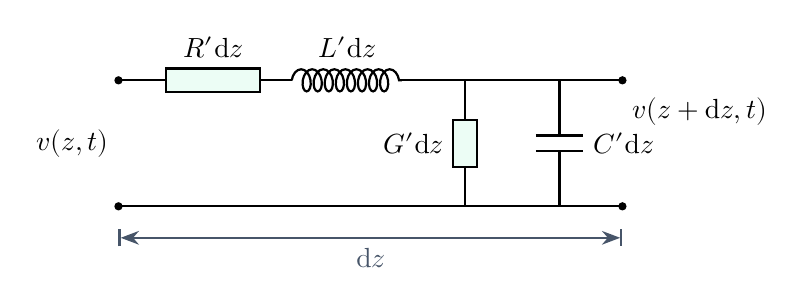
\begin{tikzpicture}[scale=1,>=Stealth,line width=0.8pt]
  \draw (0,0) -- (0.6,0); \draw (0,-1.6) -- (6.4,-1.6);
  \draw[fill=accL] (0.6,-0.15) rectangle (1.8,0.15); \node[above] at (1.2,0.15) {$R'\dd z$};
  \draw (1.8,0) -- (2.2,0);
  \draw[decorate,decoration={coil,aspect=0.6,segment length=4pt,amplitude=4pt}] (2.2,0) -- (3.6,0); \node[above] at (2.9,0.15) {$L'\dd z$};
  \draw (3.6,0) -- (6.4,0);
  \draw (4.4,0) -- (4.4,-0.5); \draw[fill=accL] (4.25,-0.5) rectangle (4.55,-1.1); \draw (4.4,-1.1) -- (4.4,-1.6);
  \node[left] at (4.25,-0.8) {$G'\dd z$};
  \draw (5.6,0) -- (5.6,-0.7); \draw (5.3,-0.7) -- (5.9,-0.7); \draw (5.3,-0.9) -- (5.9,-0.9); \draw (5.6,-0.9) -- (5.6,-1.6);
  \node[right] at (5.9,-0.8) {$C'\dd z$};
  \fill (0,0) circle (1.5pt) (0,-1.6) circle (1.5pt) (6.4,0) circle (1.5pt) (6.4,-1.6) circle (1.5pt);
  \node[left] at (0,-0.8) {$v(z,t)$}; \node[right] at (6.4,-0.4) {$v(z+\dd z,t)$};
  \draw[|<->|,gry] (0,-2.0) -- (6.4,-2.0) node[midway,below] {$\dd z$};
\end{tikzpicture}
\end{center}
\begin{donde}
\sym{R'}{resistencia de los conductores por metro (pérdidas óhmicas, efecto pelicular)}{\si{\ohm\per\metre}}
\sym{L'}{inductancia por metro (campo magnético entre conductores)}{\si{\henry\per\metre}}
\sym{G'}{conductancia del dieléctrico por metro (pérdidas en el aislante)}{\si{\siemens\per\metre}}
\sym{C'}{capacidad por metro entre los conductores}{\si{\farad\per\metre}}
\end{donde}

\subsection{Ecuaciones del telegrafista}
Aplicando las leyes de Kirchhoff al trozo y haciendo $\dd z \to 0$, en fasores:
\begin{equation}
  \frac{\dd V}{\dd z} = -(R' + \jj\omega L')\,I, \qquad \frac{\dd I}{\dd z} = -(G' + \jj\omega C')\,V .
\end{equation}
La primera dice que la tensión cae a lo largo de la línea por la impedancia serie; la segunda, que la corriente se pierde por la
admitancia paralelo. Derivando la primera y sustituyendo la segunda se obtiene la \textbf{ecuación de onda}:
\begin{equation}
  \frac{\dd^2 V}{\dd z^2} = \gamma^2 V, \qquad \gamma = \sqrt{(R' + \jj\omega L')(G' + \jj\omega C')} = \alpha + \jj\beta .
\end{equation}
\begin{donde}
\sym{\gamma}{constante de propagación (compleja)}{\si{\per\metre}}
\sym{\alpha}{constante de atenuación: cuánto se reduce la amplitud por metro}{\si{\neper\per\metre}}
\sym{\beta}{constante de fase: cuánto gira la fase por metro, $\beta = 2\pi/\lambda$}{\si{\radian\per\metre}}
\end{donde}

\subsection{Solución: dos ondas}
La solución general es la suma de una onda que viaja hacia $+z$ (hacia la carga) y otra hacia $-z$ (hacia el generador):
\begin{equation}
  V(z) = V^{+}\ee^{-\gamma z} + V^{-}\ee^{+\gamma z}, \qquad I(z) = \frac{V^{+}}{Z_0}\ee^{-\gamma z} - \frac{V^{-}}{Z_0}\ee^{+\gamma z}.
\end{equation}
\begin{donde}
\sym{V^{+}}{amplitud compleja de la onda incidente (viaja hacia la carga)}{\si{\volt}}
\sym{V^{-}}{amplitud compleja de la onda reflejada (vuelve hacia el generador)}{\si{\volt}}
\sym{\ee^{-\gamma z}}{$=\ee^{-\alpha z}\,\ee^{-\jj\beta z}$: se atenúa ($\alpha$) y se retrasa en fase ($\beta$) al avanzar}{---}
\end{donde}
El signo menos de la corriente reflejada es clave: la onda reflejada lleva la corriente en sentido contrario.

\section{Impedancia característica}
\begin{definicion}{impedancia característica $Z_0$}
Es el cociente tensión/corriente de \emph{una sola onda} viajera:
\begin{equation}
  Z_0 = \frac{V^{+}}{I^{+}} = \sqrt{\frac{R' + \jj\omega L'}{G' + \jj\omega C'}} \;\xrightarrow{\text{sin pérdidas}}\; \sqrt{\frac{L'}{C'}} .
\end{equation}
\begin{donde}
\sym{Z_0}{impedancia característica de la línea}{\si{\ohm}}
\end{donde}
\end{definicion}
\begin{atencion}{$Z_0$ no es una resistencia que se mida con un óhmetro}
Un coaxial de \SI{50}{\ohm} medido en continua da circuito abierto. $Z_0$ es la relación que impone la geometría entre $V$ e $I$ de
una onda. Si una línea infinitamente larga (o terminada en $Z_0$) se ve desde la entrada, presenta exactamente $Z_0$: la onda
entra y nunca vuelve.
\end{atencion}

En una línea sin pérdidas ($R' = G' = 0$): $\alpha = 0$, $\beta = \omega\sqrt{L'C'}$ y $v_p = 1/\sqrt{L'C'}$.
Para un coaxial de diámetros $d$ (interior) y $D$ (exterior):
\begin{equation}
  Z_0 = \frac{60}{\sqrt{\varepsilon_r}}\ln\frac{D}{d} .
\end{equation}
Por ejemplo, RG-58 ($d=\SI{0.9}{\milli\metre}$, $D = \SI{2.95}{\milli\metre}$, $\varepsilon_r \approx 2.25$) da $Z_0 \approx \CoaxZ~\si{\ohm}$.

\section{Impedancia de entrada}

Situamos la carga en $z = 0$ y medimos la distancia $d$ hacia el generador. El coeficiente de reflexión en la carga es
$\Gamma_L = V^-/V^+$ (capítulo siguiente). Dividiendo $V$ entre $I$ a la distancia $d$ se obtiene la fórmula central de la teoría de líneas:
\begin{equation}
  \boxed{\;Z_{in}(d) = Z_0\,\frac{Z_L + Z_0\tanh(\gamma d)}{Z_0 + Z_L\tanh(\gamma d)}\;}
  \;\xrightarrow{\text{sin pérdidas}}\;
  Z_0\,\frac{Z_L + \jj Z_0\tan(\beta d)}{Z_0 + \jj Z_L\tan(\beta d)} .
\end{equation}
\begin{donde}
\sym{Z_{in}(d)}{impedancia que se ve mirando hacia la carga a una distancia $d$ de ella}{\si{\ohm}}
\sym{Z_L}{impedancia de carga}{\si{\ohm}}
\sym{d}{distancia desde la carga hacia el generador}{\si{\metre}}
\sym{\beta d = \theta}{longitud eléctrica}{rad}
\end{donde}

\subsection{Casos particulares que hay que saber de memoria}
\begin{itemize}
\item \textbf{Carga adaptada} ($Z_L = Z_0$): $Z_{in} = Z_0$ para cualquier longitud.
\item \textbf{Cortocircuito} ($Z_L = 0$): $Z_{in} = \jj Z_0\tan\beta d$. Puramente reactiva: inductiva para $d < \lambda/4$.
\item \textbf{Circuito abierto} ($Z_L\to\infty$): $Z_{in} = -\jj Z_0\cot\beta d$. Capacitiva para $d < \lambda/4$.
\item \textbf{Línea de $\lambda/2$}: $\tan\beta d = 0$, así que $Z_{in} = Z_L$. La línea «se hace invisible» (a esa frecuencia).
\item \textbf{Transformador de $\lambda/4$}: $\tan\beta d \to \infty$, de donde
\begin{equation}
  Z_{in} = \frac{Z_0^2}{Z_L} .
\end{equation}
Un cortocircuito se convierte en circuito abierto y viceversa. Sirve para adaptar dos resistencias $R_1$ y $R_2$ con $Z_0 = \sqrt{R_1R_2}$.
\end{itemize}

\begin{intuicion}[: por qué una línea transforma impedancias]
En cada punto la tensión total es la suma de la onda incidente y la reflejada, que tienen fases distintas según la posición.
Al alejarse de la carga, la onda incidente se adelanta y la reflejada se retrasa: su desfase relativo cambia $2\beta d$. Por eso el
cociente $V/I$ (la impedancia) va cambiando punto a punto y se repite cada $\lambda/2$.
\end{intuicion}

\section{Ondas estacionarias}

El módulo de la tensión total a lo largo de la línea sin pérdidas es
\begin{equation}
  \abs{V(d)} = \abs{V^+}\,\abs{1 + \Gamma_L\,\ee^{-\jj 2\beta d}} .
\end{equation}
Cuando la onda reflejada está en fase con la incidente se suman ($\abs{V}_{\max} = \abs{V^+}(1+\abs{\Gamma_L})$); medio periodo
espacial ($\lambda/4$) después se restan ($\abs{V}_{\min} = \abs{V^+}(1 - \abs{\Gamma_L})$). El cociente es la ROE (VSWR):
\begin{equation}
  \mathrm{VSWR} = \frac{\abs{V}_{\max}}{\abs{V}_{\min}} = \frac{1 + \abs{\Gamma_L}}{1 - \abs{\Gamma_L}} .
\end{equation}

\begin{figure}[h]\centering
\includegraphics[width=0.85\linewidth]{generado/onda_estacionaria.pdf}
\caption{Patrón de onda estacionaria: los máximos y mínimos se repiten cada $\lambda/2$ y están separados $\lambda/4$.}
\end{figure}

\section{Pérdidas}

Con pérdidas pequeñas ($R' \ll \omega L'$, $G' \ll \omega C'$):
\begin{equation}
  \alpha \approx \frac{R'}{2Z_0} + \frac{G' Z_0}{2} = \alpha_c + \alpha_d .
\end{equation}
\begin{donde}
\sym{\alpha_c}{atenuación por los conductores; crece aproximadamente con $\sqrt f$ por el efecto pelicular}{\si{\neper\per\metre}}
\sym{\alpha_d}{atenuación por el dieléctrico; crece aproximadamente con $f$}{\si{\neper\per\metre}}
\end{donde}
La atenuación total de una línea de longitud $\ell$ es $A = 8.686\,\alpha\,\ell$ dB. Además, la reflexión «pierde» dos veces:
la onda reflejada se atenúa a la ida y a la vuelta, de modo que en la entrada $\abs{\Gamma_{in}} = \abs{\Gamma_L}\ee^{-2\alpha\ell}$.
Una línea con muchas pérdidas \emph{parece} bien adaptada aunque la carga no lo esté: es un efecto engañoso al medir antenas al final de un cable largo.

\begin{ejemplo}{coaxial de \SI{3.2}{\metre} a \SI{145}{\mega\hertz}}
$Z_0 = \SI{50}{\ohm}$, $v_f = 0.66$, sin pérdidas, carga $Z_L = 100 + \jj 50\,\si{\ohm}$:
\begin{align*}
  \lambda &= \frac{0.66\,c}{\SI{145}{\mega\hertz}} = \LnLam~\si{\metre}, \qquad \beta = \frac{2\pi}{\lambda} = \LnBeta~\si{\radian\per\metre}\\
  \theta &= \beta\ell = \LnTheta^\circ \quad(\ell = \LnLenLam\,\lambda)\\
  \Gamma_L &= \frac{Z_L - Z_0}{Z_L + Z_0} = \LnGl, \qquad \mathrm{VSWR} = \LnVswr\\
  \abs{V}_{\max} / \abs{V^+} &= \LnVmax, \qquad \abs{V}_{\min}/\abs{V^+} = \LnVmin\\
  Z_{in} &= \LnZin~\si{\ohm}
\end{align*}
El VSWR no cambia a lo largo de la línea sin pérdidas, pero la impedancia de entrada sí, y mucho.
\end{ejemplo}

\begin{enlaapp}
El módulo \app{Transmission Lines} calcula $\lambda$, $\beta$, $\theta$, $Z_{in}$, $\Gamma$ y VSWR para cualquier línea definida por $Z_0$ y $v_f$,
obtiene $Z_0$ a partir de la geometría para coaxial, par de hilos y microstrip, y admite pérdidas definidas en dB/m (y escaladas con $\sqrt f$ y $f$). Muestra además el patrón de onda estacionaria y
dibuja en la carta de Smith la rotación de $\Gamma$ al recorrer la línea.
\end{enlaapp}

\chapter{Reflexión y carta de Smith}\label{cap:smith}

\section{El coeficiente de reflexión}

Cuando una onda llega a una carga $Z_L$ distinta de $Z_0$, la carga impone su propia relación $V/I$. La única forma de cumplirla
es que aparezca una onda reflejada. En la carga ($d = 0$): $V = V^+ + V^-$ e $I = (V^+ - V^-)/Z_0$. Imponiendo $V/I = Z_L$:
\begin{equation}
  Z_L = Z_0\,\frac{V^+ + V^-}{V^+ - V^-} \quad\Longrightarrow\quad
  \boxed{\;\Gamma_L = \frac{V^-}{V^+} = \frac{Z_L - Z_0}{Z_L + Z_0}\;}
\end{equation}
\begin{donde}
\sym{\Gamma_L}{coeficiente de reflexión en la carga (complejo): qué fracción de la onda vuelve y con qué fase}{---}
\sym{Z_L}{impedancia de carga}{\si{\ohm}}
\sym{Z_0}{impedancia de referencia (la de la línea o del sistema, casi siempre \SI{50}{\ohm})}{\si{\ohm}}
\end{donde}
Y la relación inversa, que permite pasar de una medida de $\Gamma$ a una impedancia:
\begin{equation}
  Z_L = Z_0\,\frac{1 + \Gamma_L}{1 - \Gamma_L}.
\end{equation}

\subsection{Valores de referencia}
\begin{center}
\begin{tabular}{lccc}\toprule
Carga & $Z_L$ & $\Gamma_L$ & Interpretación \\ \midrule
Adaptada & $Z_0$ & $0$ & no hay onda reflejada \\
Cortocircuito & $0$ & $-1 = 1\angle 180^\circ$ & todo vuelve, con la tensión invertida \\
Circuito abierto & $\infty$ & $+1 = 1\angle 0^\circ$ & todo vuelve, con la misma tensión \\
Reactancia pura & $\jj X$ & $\abs{\Gamma} = 1$ & todo vuelve, con una fase intermedia \\
Carga pasiva cualquiera & $R \ge 0$ & $\abs{\Gamma} \le 1$ & parte se absorbe, parte vuelve \\ \bottomrule
\end{tabular}
\end{center}
\begin{intuicion}[: por qué $\abs{\Gamma} \le 1$ en una carga pasiva]
Una carga pasiva no puede devolver más energía de la que recibe. La potencia reflejada es $\abs{\Gamma}^2$ veces la incidente, así que
$\abs{\Gamma}\le 1$ siempre que $R\ge0$. Un $\abs{\Gamma} > 1$ indica una resistencia negativa: un dispositivo activo que puede oscilar
(capítulo~\ref{cap:sparams}, estabilidad).
\end{intuicion}

\subsection{Reflexión a lo largo de la línea}
A una distancia $d$ de la carga, la onda incidente se ha adelantado $\beta d$ y la reflejada ha tenido que recorrer $d$ más; el cociente gira
\emph{dos veces}:
\begin{equation}
  \Gamma(d) = \Gamma_L\,\ee^{-2\gamma d} \;\xrightarrow{\text{sin pérdidas}}\; \Gamma_L\,\ee^{-\jj 2\beta d}.
\end{equation}
\begin{donde}
\sym{\Gamma(d)}{coeficiente de reflexión visto a la distancia $d$ de la carga}{---}
\sym{2\beta d}{giro de fase de ida y vuelta}{rad}
\end{donde}
En una línea sin pérdidas, $\abs{\Gamma}$ es constante y sólo gira su fase, en sentido horario, una vuelta completa cada $\lambda/2$.
Esta es la base geométrica de la carta de Smith.

\section{\texorpdfstring{Magnitudes derivadas de $\abs{\Gamma}$}{Magnitudes derivadas de |Γ|}}

\begin{definicion}{VSWR, pérdida de retorno y pérdida por desadaptación}
\begin{align}
  \mathrm{VSWR} &= \frac{1+\abs\Gamma}{1-\abs\Gamma}, \qquad \abs\Gamma = \frac{\mathrm{VSWR}-1}{\mathrm{VSWR}+1}\\
  RL &= -20\log_{10}\abs\Gamma \quad [\si{\decibel}]\\
  ML &= -10\log_{10}\left(1 - \abs\Gamma^2\right) \quad [\si{\decibel}]
\end{align}
\begin{donde}
\sym{\mathrm{VSWR}}{relación de onda estacionaria (ROE): de 1 (perfecta) a $\infty$ (reflexión total)}{---}
\sym{RL}{return loss: cuántos dB por debajo de la incidente está la onda reflejada. \textbf{Cuanto mayor, mejor}}{\si{\decibel}}
\sym{ML}{mismatch loss: potencia que \emph{no} llega a la carga por culpa de la reflexión}{\si{\decibel}}
\sym{\abs\Gamma^2}{fracción de potencia reflejada}{---}
\sym{1-\abs\Gamma^2}{fracción de potencia entregada a la carga}{---}
\end{donde}
\end{definicion}

\begin{atencion}{el signo de la return loss}
La return loss es positiva: $RL = \SI{20}{\decibel}$ significa $\abs\Gamma = 0.1$. Lo que se representa en un VNA es $\abs{S_{11}}$ en dB,
que es \emph{negativo}: $\abs{S_{11}}_{\si{\decibel}} = -RL$. Decir «una return loss de \SI{-20}{\decibel}» es técnicamente incorrecto,
aunque muy común.
\end{atencion}

\begin{center}
\small
\begin{tabular}{cccccc}\toprule
VSWR & $\abs\Gamma$ & $RL$ (dB) & Reflejada (\%) & Entregada (\%) & $ML$ (dB)\\ \midrule
\tabla{generado/tabla_vswr.tex}
\bottomrule
\end{tabular}
\end{center}
Observe que un VSWR de 2 (que parece «malo») sólo pierde \SI{0.51}{\decibel}: la ROE es sobre todo un problema de potencia reflejada hacia
el transmisor y de tensiones elevadas en la línea, más que de pérdida de señal.

\begin{ejemplo}{$Z_L = 80 + \jj 30\,\si{\ohm}$ en un sistema de \SI{50}{\ohm}}
\begin{align*}
  z &= \frac{Z_L}{Z_0} = \GejZn\\
  \Gamma &= \frac{Z_L - Z_0}{Z_L + Z_0} = \frac{30 + \jj30}{130 + \jj30} = \GejRect = \GejPol\\
  \mathrm{VSWR} &= \frac{1 + \GejMag}{1 - \GejMag} = \GejVswr\\
  RL &= \GejRl~\si{\decibel}, \qquad ML = \GejMl~\si{\decibel}, \qquad \text{potencia reflejada} = \GejRefl~\%
\end{align*}
\end{ejemplo}

\subsection{Fuentes complejas: ondas de potencia}
Si la fuente no es una resistencia pura de valor $Z_0$, la reflexión que importa para la potencia entregada es la de \emph{onda de potencia}
(Kurokawa):
\begin{equation}
  \Gamma_p = \frac{Z_L - \conj{Z_s}}{Z_L + Z_s} .
\end{equation}
\begin{donde}
\sym{\Gamma_p}{coeficiente de reflexión de onda de potencia}{---}
\sym{Z_s}{impedancia de la fuente}{\si{\ohm}}
\end{donde}
Es cero exactamente cuando $Z_L = \conj{Z_s}$ (máxima transferencia de potencia) y $1 - \abs{\Gamma_p}^2$ es la fracción de la potencia
\emph{disponible} que llega a la carga. Cuando $Z_s = Z_0$ es real, coincide con el $\Gamma$ habitual.

\section{La carta de Smith}

\subsection{La idea}
La carta de Smith es el plano complejo de $\Gamma$ (el disco $\abs\Gamma\le1$) sobre el que se dibujan las curvas de resistencia y
reactancia normalizadas constantes. Así, un mismo punto se lee a la vez como $\Gamma$ (posición) y como $Z$ (rejilla).

Con la impedancia normalizada $z = Z/Z_0 = r + \jj x$, la relación es una \emph{transformación de Möbius}:
\begin{equation}
  \Gamma = \frac{z - 1}{z + 1}, \qquad z = \frac{1 + \Gamma}{1 - \Gamma}.
\end{equation}
\begin{donde}
\sym{z = r + \jj x}{impedancia normalizada (adimensional)}{---}
\sym{r}{resistencia normalizada $R/Z_0$}{---}
\sym{x}{reactancia normalizada $X/Z_0$}{---}
\end{donde}

\subsection{Derivación de los círculos}
Escribimos $\Gamma = u + \jj v$ y separamos parte real e imaginaria de $z = (1+\Gamma)/(1-\Gamma)$, multiplicando por el conjugado del denominador:
\begin{equation}
  r = \frac{1 - u^2 - v^2}{(1-u)^2 + v^2}, \qquad x = \frac{2v}{(1-u)^2 + v^2}.
\end{equation}
Reordenando cada una como ecuación de una circunferencia $(u - u_c)^2 + (v - v_c)^2 = \rho^2$:
\begin{align}
  \text{$r$ constante:}\quad & \left(u - \frac{r}{1+r}\right)^2 + v^2 = \left(\frac{1}{1+r}\right)^2 \\
  \text{$x$ constante:}\quad & (u - 1)^2 + \left(v - \frac1x\right)^2 = \left(\frac1x\right)^2
\end{align}
\begin{donde}
\sym{u, v}{partes real e imaginaria de $\Gamma$ (coordenadas del punto en la carta)}{---}
\sym{\frac{r}{1+r},\ \frac1{1+r}}{centro sobre el eje real y radio de cada círculo de resistencia}{---}
\sym{(1, \frac1x),\ \frac1{\abs x}}{centro y radio de cada arco de reactancia}{---}
\end{donde}
Todos los círculos de $r$ constante pasan por el punto $\Gamma = 1$ (circuito abierto) y todos los de $x$ constante también: ese punto
es la imagen de $z = \infty$.

\begin{figure}[h]\centering
\includegraphics[width=0.62\linewidth]{generado/smith_regiones.pdf}
\caption{Regiones de la carta de Smith: mitad superior inductiva ($x>0$), mitad inferior capacitiva ($x<0$), eje horizontal resistivo puro,
centro adaptado ($z = 1$), extremo izquierdo cortocircuito, extremo derecho circuito abierto.}
\end{figure}

\subsection{Cómo leer la carta}
\begin{itemize}
\item \textbf{Distancia al centro} $=\abs\Gamma$: los círculos concéntricos con el centro son de VSWR constante.
\item \textbf{Ángulo} $=$ fase de $\Gamma$, medida desde el eje real positivo.
\item \textbf{Moverse por una línea sin pérdidas} hacia el generador es girar en sentido \emph{horario} sobre un círculo de VSWR constante;
una vuelta completa son $\lambda/2$. Con pérdidas, el punto describe una espiral hacia el centro.
\item \textbf{Añadir una reactancia en serie} mueve el punto sobre su círculo de $r$ constante (hacia arriba si es una bobina, hacia abajo si es un condensador).
\item \textbf{Añadir una susceptancia en paralelo} mueve el punto sobre un círculo de $g$ constante de la carta de admitancias.
\end{itemize}

\subsection{La carta de admitancias}
Como $y = 1/z$, se cumple
\begin{equation}
  \Gamma_y = \frac{y - 1}{y + 1} = \frac{1/z - 1}{1/z + 1} = -\,\frac{z-1}{z+1} = -\Gamma .
\end{equation}
Es decir, \textbf{la admitancia de un punto se lee en el punto diametralmente opuesto} (girado $180^\circ$). La carta de admitancias es la
de impedancias girada media vuelta; superponer las dos (carta «ZY») permite trabajar con elementos en serie y en paralelo a la vez.

\begin{figure}[h]\centering
\includegraphics[width=0.62\linewidth]{generado/smith_ejemplo.pdf}
\caption{El ejemplo $Z_L = 80 + \jj30\,\si{\ohm}$ en la carta: la flecha es el vector $\Gamma$ y el círculo discontinuo reúne todos los puntos con el mismo VSWR (los que se recorren al añadir línea sin pérdidas).}
\end{figure}

\begin{enlaapp}
La \app{Smith Chart} es SVG propio: dibuja las rejillas Z, Y o ZY, círculos de VSWR, marcadores con lectura simultánea de $z$, $y$, $\Gamma$,
VSWR y RL, trazas de medidas o archivos Touchstone y trayectorias de redes de adaptación. Se exporta como SVG o PNG de 4000 píxeles.
En el \app{Circuit Builder} cada elemento que se añade a la escalera dibuja su arco (círculo $r$ constante si es serie, círculo $g$ constante si es paralelo).
\end{enlaapp}

\chapter{Adaptación de impedancias}\label{cap:adaptacion}

\section{El problema}

Tenemos una fuente de impedancia $Z_s$ (normalmente \SI{50}{\ohm}) y una carga $Z_L$ distinta. Queremos insertar entre ambas una red
\textbf{sin pérdidas} (sólo bobinas, condensadores o tramos de línea) tal que la carga, vista a través de la red, presente
$Z_{in} = \conj{Z_s}$. Como la red no disipa, toda la potencia disponible llega a la carga.

\begin{intuicion}[: por qué hacen falta dos elementos]
Una impedancia tiene dos grados de libertad ($R$ y $X$). Para llevar un punto cualquiera de la carta de Smith al centro hacen falta, en general,
dos movimientos independientes: uno que ajuste la parte real y otro que cancele la imaginaria. Por eso la red mínima tiene dos elementos (red L).
\end{intuicion}

\section{Red L}

Tiene un elemento en serie y otro en paralelo. Hay dos configuraciones según qué elemento queda junto a la carga:
\begin{itemize}
\item \textbf{Paralelo junto a la carga}: útil cuando $R_L > R_s$. El elemento en paralelo reduce la resistencia equivalente de la carga
hasta $R_s$; después el elemento serie cancela la reactancia que queda.
\item \textbf{Serie junto a la carga}: útil cuando $R_L < R_s$. El elemento serie lleva la carga al círculo donde la conductancia vale $1/R_s$
y el paralelo cancela la susceptancia restante.
\end{itemize}

\subsection{Derivación (carga resistiva, paralelo junto a la carga)}
Sea $R_L > R_s$ con cargas reales. El elemento paralelo de susceptancia $B$ y el serie de reactancia $X$ deben cumplir
\begin{equation}
  R_s = \Re\left\{\frac{1}{1/R_L + \jj B}\right\} = \frac{R_L}{1 + (BR_L)^2} \quad\Rightarrow\quad B = \pm\frac{1}{R_L}\sqrt{\frac{R_L}{R_s} - 1}.
\end{equation}
Después, el elemento serie cancela la parte imaginaria que queda: $X = \mp\sqrt{R_s(R_L - R_s)}$. Definiendo
\begin{equation}
  Q = \sqrt{\frac{R_L}{R_s} - 1}, \qquad \abs{X} = Q\,R_s, \qquad \abs{B} = \frac{Q}{R_L}.
\end{equation}
\begin{donde}
\sym{Q}{factor de calidad de la red L, fijado por el cociente de resistencias (no se puede elegir)}{---}
\sym{B}{susceptancia del elemento en paralelo ($B>0$ condensador, $B<0$ bobina)}{\si{\siemens}}
\sym{X}{reactancia del elemento en serie ($X>0$ bobina, $X<0$ condensador)}{\si{\ohm}}
\end{donde}
Los dos signos dan las dos soluciones: paso bajo (bobina serie, condensador paralelo) y paso alto (condensador serie, bobina paralelo).
Para pasar de reactancias a componentes: $L = X/\omega$, $C = -1/(\omega X)$ (serie) o $C = B/\omega$, $L = -1/(\omega B)$ (paralelo).

El motor no usa estas fórmulas cerradas para cargas complejas: resuelve directamente $\Re$ e $\Im$ de la condición $Z_{in} = \conj{Z_s}$ para
las dos configuraciones, convierte cada reactancia en componente y \textbf{verifica} cada solución recalculando $Z_{in}$ con la cascada
ABCD; las que no cumplen la condición con una tolerancia de $10^{-6}$ se descartan.

\begin{ejemplo}{carga $Z_L = 25 - \jj40\,\si{\ohm}$ a \SI{433}{\mega\hertz}, fuente de \SI{50}{\ohm}}
Antes de adaptar: $\abs{\Gamma} = \MtGb$, VSWR $=\MtVb$. Soluciones de red L encontradas por el motor:
\begin{center}\small
\begin{tabular}{clp{6.4cm}c}\toprule
\# & Topología & Elementos (desde la fuente) & BW (VSWR$\le2$)\\ \midrule
\tabla{generado/tabla_red_l.tex}
\bottomrule
\end{tabular}
\end{center}
El límite de Bode--Fano (más abajo) para esta carga es $\Delta f/f_0 \le \MtBf\,\%$ con $Q_L = \MtQl$.
\end{ejemplo}

\begin{figure}[h]\centering
\includegraphics[width=\linewidth]{generado/red_l.pdf}
\caption{Red L para $Z_L = 25 - \jj40\,\si{\ohm}$ a \SI{433}{\mega\hertz}. Izquierda: cada elemento es un arco en la carta (serie: círculo de $r$ constante; paralelo: círculo de $g$ constante). Derecha: $\abs\Gamma$ frente a la frecuencia; la adaptación sólo es perfecta en $f_0$.}
\end{figure}

\begin{ejemplo}{red L con $Z_0 = \SI{100}{\ohm}$}
Carga $200 - \jj100\,\si{\ohm}$ a \SI{500}{\mega\hertz}, fuente de \SI{100}{\ohm}. Una de las soluciones es un condensador en paralelo de
$\PozC~\si{\pico\farad}$ junto a la carga y una bobina en serie de $\PozL~\si{\nano\henry}$. (Es el problema clásico de Pozar, ejemplo 5.1, que sirve
para validar el motor.)
\end{ejemplo}

\section{Redes Pi y T: controlar el ancho de banda}
La red L tiene un $Q$ fijo. Si se quiere \emph{más} selectividad (filtrar armónicos) o elegir el ancho de banda, se usan tres elementos.
La idea es pasar por una resistencia intermedia virtual $R_v$:
\begin{equation}
  \text{Pi:}\ R_v = \frac{\max(R_s, R_L)}{1 + Q_{\text{red}}^2} < R_s, R_L, \qquad
  \text{T:}\ R_v = \min(R_s, R_L)\,(1 + Q_{\text{red}}^2) > R_s, R_L .
\end{equation}
\begin{donde}
\sym{R_v}{resistencia virtual en el nudo central (no existe físicamente)}{\si{\ohm}}
\sym{Q_{\text{red}}}{$Q$ deseado; debe ser mayor que el de la red L equivalente}{---}
\end{donde}
Una Pi son dos redes L espalda con espalda (paralelo--serie y serie--paralelo, con los dos elementos serie centrales sumados): la primera
transforma $R_L$ en $R_v$ y la segunda $R_v$ en $R_s$. Si el $Q$ pedido es menor que el mínimo $\sqrt{R_{\max}/R_{\min} - 1}$, la red no
existe y el motor lo indica. Mayor $Q$ significa menor
ancho de banda ($BW \approx f_0/Q$) y mayor sensibilidad a tolerancias.

\section{\texorpdfstring{Transformador de $\lambda/4$}{Transformador de λ/4}}
Para cargas reales: una línea de $\lambda/4$ con
\begin{equation}
  Z_T = \sqrt{Z_s\,R_L}.
\end{equation}
Si la carga es compleja, primero se añade un tramo de línea de $Z_0$ hasta que $Z$ se vuelve real (un máximo o mínimo de la onda estacionaria,
donde el punto cruza el eje horizontal de la carta) y después el transformador. El motor calcula la distancia y las dos opciones.

\section{Adaptación con stubs}

\subsection{Stub simple}
Un \emph{stub} es un tramo de línea en cortocircuito o en abierto conectado en paralelo. Se comporta como una susceptancia pura
(capítulo~\ref{cap:lineas}):
\begin{equation}
  B_{\text{stub,corto}} = -\frac{1}{Z_0}\cot\beta\ell, \qquad B_{\text{stub,abierto}} = \frac{1}{Z_0}\tan\beta\ell .
\end{equation}
El procedimiento es:
\begin{enumerate}
\item Desplazarse por la línea desde la carga una distancia $d$ hasta que la admitancia normalizada sea $y = 1 + \jj b$
(en la carta: girar hasta cortar el círculo $g = 1$).
\item En ese punto colocar un stub de longitud $\ell$ que aporte la susceptancia $-b$, de modo que $y = 1$.
\end{enumerate}
\begin{donde}
\sym{d}{distancia de la carga al punto de conexión del stub}{\si{\metre} o $\lambda$}
\sym{\ell}{longitud del stub}{\si{\metre} o $\lambda$}
\sym{b}{susceptancia normalizada que hay que cancelar}{---}
\end{donde}
Siempre hay dos soluciones (los dos cortes con el círculo $g=1$ en una vuelta).
\begin{ejemplo}{stub en cortocircuito, $Z_L = 60 - \jj80\,\si{\ohm}$ a \SI{2}{\giga\hertz}}
Soluciones del motor: $d = \StD\,\lambda$, $\ell = \StL\,\lambda$, o bien $d = \StDb\,\lambda$, $\ell = \StLb\,\lambda$.
\end{ejemplo}

\subsection{Doble stub}
Con stubs en posiciones fijas (el primero a una distancia $d_1$ de la carga y el segundo separado $\lambda/8$, por ejemplo) la adaptación se consigue ajustando sólo sus longitudes. Su inconveniente:
existe una \emph{zona prohibida} de cargas que no se pueden adaptar con una separación dada; el motor lo detecta e informa.

\section{Límite de Bode--Fano}

\begin{definicion}{límite de Bode--Fano}
Para una carga que se modela como $R$ y $X$ en serie (con $Q_L = \abs{X_L}/R_L$), ninguna red sin pérdidas, por compleja que sea, puede
conseguir una reflexión $\abs\Gamma \le \Gamma_m$ en una banda relativa mayor que
\begin{equation}
  \frac{\Delta f}{f_0} \le \frac{\pi}{Q_L\,\ln(1/\Gamma_m)} .
\end{equation}
\begin{donde}
\sym{\Delta f/f_0}{ancho de banda relativo alcanzable}{---}
\sym{Q_L}{factor de calidad de la carga a $f_0$}{---}
\sym{\Gamma_m}{máxima reflexión tolerada en la banda (por ejemplo $1/3$ para VSWR 2)}{---}
\end{donde}
\end{definicion}
\begin{intuicion}[: no se puede tener todo]
Una carga muy reactiva (alto $Q_L$) almacena mucha energía, y eso limita lo ancha que puede ser la adaptación. Si se exige reflexión muy baja
($\Gamma_m\to 0$, $\ln(1/\Gamma_m)\to\infty$), el ancho de banda tiende a cero. Bode--Fano es un \emph{techo teórico}: dice cuándo dejar de
buscar una red mejor.
\end{intuicion}

\section{Tolerancias y Monte Carlo}
Los componentes reales tienen tolerancia (por ejemplo $\pm5\,\%$) y valores comerciales (series E12, E24). La aplicación:
\begin{enumerate}
\item Redondea los valores ideales a la serie E elegida y recalcula la respuesta.
\item Ejecuta un análisis Monte Carlo: genera $N$ redes (de 10 a \num{20000}) variando cada $L$, $C$ y longitud de línea dentro de su
tolerancia, con distribución uniforme o gaussiana (en la gaussiana la tolerancia se toma como $3\sigma$). Para cada red calcula el VSWR en
toda la banda y presenta: media, desviación típica, percentiles 5/50/95 (envolvente), histograma en $f_0$ y \emph{rendimiento} (yield),
la fracción de unidades con VSWR$(f_0)$ dentro del objetivo.
\end{enumerate}

\begin{enlaapp}
El \app{Matching Designer} implementa red L, Pi, T, $\lambda/4$, stub simple y doble stub, con factor $Q$ finito de los componentes, barrido en
frecuencia de cada solución, ancho de banda medido, límite de Bode--Fano, trayectoria en la carta de Smith, redondeo a series E y Monte Carlo.
\end{enlaapp}

\chapter{Parámetros S, redes y estabilidad}\label{cap:sparams}

\section{Por qué parámetros S}

Los parámetros Z, Y, H o ABCD se miden con circuitos abiertos o cortocircuitos en los puertos. En RF eso es imposible: un abierto
radia y tiene capacidad parásita, un corto tiene inductancia, y un transistor puede oscilar con esas terminaciones. Los parámetros S
(\emph{scattering}, de dispersión) se miden con todos los puertos terminados en $Z_0$ y relacionan \textbf{ondas}, que es justo lo que mide un VNA.

\section{Ondas de potencia}
\begin{definicion}{ondas $a$ y $b$}
En cada puerto $i$ con tensión $V_i$ y corriente $I_i$ (entrante), y una referencia real $Z_0$:
\begin{equation}
  a_i = \frac{V_i + Z_0 I_i}{2\sqrt{Z_0}}, \qquad b_i = \frac{V_i - Z_0 I_i}{2\sqrt{Z_0}} .
\end{equation}
\begin{donde}
\sym{a_i}{onda incidente en el puerto $i$ (entra en la red)}{$\sqrt{\mathrm{W}}$}
\sym{b_i}{onda reflejada o emergente del puerto $i$ (sale de la red)}{$\sqrt{\mathrm{W}}$}
\sym{\abs{a_i}^2}{potencia incidente (con valores eficaces)}{\si{\watt}}
\end{donde}
\end{definicion}
Comparando con el capítulo~\ref{cap:lineas}: $a_i = V_i^+/\sqrt{Z_0}$ y $b_i = V_i^-/\sqrt{Z_0}$. Dividir por $\sqrt{Z_0}$ hace que
$\abs{a}^2$ sea directamente una potencia.

\section{La matriz S}
\begin{definicion}{matriz de dispersión}
\begin{equation}
  \mathbf{b} = \mathbf{S}\,\mathbf{a}, \qquad
  \begin{pmatrix} b_1 \\ b_2 \end{pmatrix} = \begin{pmatrix} S_{11} & S_{12} \\ S_{21} & S_{22} \end{pmatrix}\begin{pmatrix} a_1 \\ a_2 \end{pmatrix},
  \qquad S_{ij} = \left.\frac{b_i}{a_j}\right|_{a_k = 0,\ k\ne j}.
\end{equation}
\begin{donde}
\sym{S_{ij}}{respuesta que sale por el puerto $i$ cuando se excita sólo el puerto $j$ y los demás están terminados en $Z_0$}{---}
\sym{S_{11}, S_{22}}{coeficientes de reflexión de entrada y de salida (con el otro puerto adaptado)}{---}
\sym{S_{21}}{transmisión directa: ganancia o pérdida de inserción}{---}
\sym{S_{12}}{transmisión inversa: aislamiento}{---}
\end{donde}
\end{definicion}
Notación del primer subíndice: \emph{dónde se mide}; del segundo: \emph{dónde se excita}. $S_{21}$ se lee «del 1 al 2».

\subsection{Magnitudes habituales}
\begin{align}
  IL &= -20\log_{10}\abs{S_{21}} \quad\text{(pérdida de inserción, positiva)}\\
  G &= 20\log_{10}\abs{S_{21}} \quad\text{(ganancia, para amplificadores)}\\
  \tau_g &= -\frac{\dd\phi_{21}}{\dd\omega} = -\frac{1}{2\pi}\frac{\dd\phi_{21}}{\dd f}
\end{align}
\begin{donde}
\sym{\phi_{21}}{fase de $S_{21}$, desenrollada (sin saltos de $360^\circ$)}{rad}
\sym{\tau_g}{retardo de grupo: tiempo que tarda la envolvente de una señal en atravesar la red}{\si{\second}}
\end{donde}
\begin{intuicion}[: retardo de grupo]
Si la fase cae linealmente con la frecuencia, todas las componentes de una señal llegan con el mismo retardo y la forma se conserva.
Un retardo de grupo variable en la banda distorsiona señales de banda ancha (es la razón por la que se especifica la «planitud» del
retardo de grupo en filtros).
\end{intuicion}

\subsection{Propiedades de redes físicas}
\begin{itemize}
\item \textbf{Recíproca} (sin ferritas ni elementos activos): $\mathbf S = \mathbf S^T$, es decir, $S_{12} = S_{21}$.
\item \textbf{Sin pérdidas}: $\mathbf S^H\mathbf S = \mathbf I$ (matriz unitaria). Para dos puertos: $\abs{S_{11}}^2 + \abs{S_{21}}^2 = 1$.
\item \textbf{Pasiva}: los autovalores de $\mathbf S^H\mathbf S$ son $\le 1$; ninguna combinación de entradas devuelve más potencia de la que recibe.
\end{itemize}
La cantidad $1 - \abs{S_{11}}^2 - \abs{S_{21}}^2$ es la fracción de potencia disipada (o radiada) en la red.

\section{Conversión entre representaciones}
Con $Z_0$ real igual en todos los puertos y $\mathbf I$ la matriz identidad:
\begin{equation}
  \mathbf S = (\mathbf Z - Z_0\mathbf I)(\mathbf Z + Z_0\mathbf I)^{-1}, \qquad \mathbf Z = Z_0(\mathbf I + \mathbf S)(\mathbf I - \mathbf S)^{-1}.
\end{equation}
Es la generalización matricial de $\Gamma = (Z - Z_0)/(Z + Z_0)$. Para admitancias, con $Y_0 = 1/Z_0$:
$\mathbf S = (Y_0\mathbf I - \mathbf Y)(Y_0\mathbf I + \mathbf Y)^{-1}$. El motor convierte H y G a S con las fórmulas cerradas de Frickey
(válidas para dos puertos) y comprueba todas las conversiones contra scikit-rf en los tests.

\subsection{Matriz ABCD y cascadas}
\begin{definicion}{parámetros de transmisión}
\begin{equation}
  \begin{pmatrix} V_1 \\ I_1 \end{pmatrix} = \begin{pmatrix} A & B \\ C & D \end{pmatrix}\begin{pmatrix} V_2 \\ -I_2 \end{pmatrix}.
\end{equation}
\begin{donde}
\sym{A}{relación de tensiones con salida en abierto, $V_1/V_2$}{---}
\sym{B}{impedancia de transferencia con salida en corto}{\si{\ohm}}
\sym{C}{admitancia de transferencia con salida en abierto}{\si{\siemens}}
\sym{D}{relación de corrientes con salida en corto}{---}
\end{donde}
\end{definicion}
Su gran ventaja: \textbf{la red total de una cascada es el producto de las matrices}, en orden desde la entrada:
\begin{equation}
  \mathbf T_{\text{total}} = \mathbf T_1\,\mathbf T_2\cdots\mathbf T_n .
\end{equation}
Los bloques básicos son:
\begin{equation}
  \underbrace{\begin{pmatrix} 1 & Z \\ 0 & 1\end{pmatrix}}_{\text{serie } Z}, \qquad
  \underbrace{\begin{pmatrix} 1 & 0 \\ Y & 1\end{pmatrix}}_{\text{paralelo } Y}, \qquad
  \underbrace{\begin{pmatrix} \cosh\gamma\ell & Z_0\sinh\gamma\ell \\ \sinh(\gamma\ell)/Z_0 & \cosh\gamma\ell\end{pmatrix}}_{\text{línea}} .
\end{equation}
Y la impedancia de entrada con una carga $Z_L$ al final es
\begin{equation}
  Z_{in} = \frac{A Z_L + B}{C Z_L + D}.
\end{equation}
\begin{enlaapp}
Así funciona por dentro el \app{Circuit Builder} y la verificación del \app{Matching Designer}: cada elemento (serie, paralelo, línea, stub)
es una matriz ABCD por frecuencia, se multiplican todas y se aplica la fórmula de $Z_{in}$. Los puntos intermedios de la cascada dan los
arcos dibujados en la carta de Smith.
\end{enlaapp}

\section{Reflexión de entrada con carga arbitraria}
Si el puerto 2 no está terminado en $Z_0$ sino en una carga con coeficiente $\Gamma_L$, entonces $a_2 = \Gamma_L b_2$ y despejando:
\begin{equation}
  \Gamma_{in} = S_{11} + \frac{S_{12}S_{21}\Gamma_L}{1 - S_{22}\Gamma_L}, \qquad
  \Gamma_{out} = S_{22} + \frac{S_{12}S_{21}\Gamma_S}{1 - S_{11}\Gamma_S}.
\end{equation}
\begin{donde}
\sym{\Gamma_L, \Gamma_S}{coeficientes de reflexión de la carga y de la fuente, referidos a $Z_0$}{---}
\sym{\Gamma_{in}, \Gamma_{out}}{reflexión vista en la entrada y en la salida del dispositivo}{---}
\end{donde}
El segundo término es la «realimentación» a través de $S_{12}$: sólo si $S_{12} = 0$ (red unilateral) la entrada no depende de la carga.

\section{Estabilidad de amplificadores}

Un amplificador es \textbf{inestable} si para alguna carga o fuente pasiva ($\abs{\Gamma_L}, \abs{\Gamma_S} < 1$) resulta
$\abs{\Gamma_{in}} > 1$ o $\abs{\Gamma_{out}} > 1$: presenta resistencia negativa y puede oscilar.

\begin{definicion}{criterios de estabilidad incondicional}
\begin{align}
  \Delta &= S_{11}S_{22} - S_{12}S_{21}\\
  K &= \frac{1 - \abs{S_{11}}^2 - \abs{S_{22}}^2 + \abs{\Delta}^2}{2\,\abs{S_{12}S_{21}}} > 1 \quad\text{y}\quad \abs\Delta < 1\\
  \mu &= \frac{1 - \abs{S_{11}}^2}{\abs{S_{22} - \Delta\conj{S_{11}}} + \abs{S_{12}S_{21}}} > 1
\end{align}
\begin{donde}
\sym{\Delta}{determinante de la matriz S}{---}
\sym{K}{factor de Rollett; necesita además la condición $\abs\Delta<1$}{---}
\sym{\mu}{factor de Edwards--Sinsky: condición necesaria y suficiente por sí sola; además, cuanto mayor, más margen}{---}
\end{donde}
\end{definicion}
\begin{intuicion}[: qué mide $\mu$]
$\mu$ es la distancia desde el centro de la carta de $\Gamma_L$ hasta la región inestable más cercana. $\mu > 1$ significa que toda la carta
(todas las cargas pasivas) queda en zona estable. Por eso la aplicación lo usa como indicador principal.
\end{intuicion}

\subsection{Círculos de estabilidad}
El lugar de las cargas $\Gamma_L$ que dan exactamente $\abs{\Gamma_{in}} = 1$ es una circunferencia en el plano $\Gamma_L$:
\begin{equation}
  C_L = \frac{\conj{\left(S_{22} - \Delta\conj{S_{11}}\right)}}{\abs{S_{22}}^2 - \abs\Delta^2}, \qquad
  r_L = \abs{\frac{S_{12}S_{21}}{\abs{S_{22}}^2 - \abs\Delta^2}} .
\end{equation}
\begin{donde}
\sym{C_L, r_L}{centro (complejo) y radio del círculo de estabilidad de salida}{---}
\end{donde}
Para saber qué lado es estable basta un punto de prueba: el centro de la carta ($\Gamma_L = 0$) da $\abs{\Gamma_{in}} = \abs{S_{11}}$; si es
menor que 1, el lado del círculo que contiene el origen es el estable. Análogamente para la fuente ($C_S$, $r_S$, intercambiando 1 y 2).

\begin{ejemplo}{transistor de microondas (datos de ejemplo)}
$S_{11} = 0.894\angle{-60.6^\circ}$, $S_{12} = 0.020\angle 62.4^\circ$, $S_{21} = 3.122\angle 123.6^\circ$, $S_{22} = 0.781\angle{-27.6^\circ}$:
\[
  K = \StbK, \qquad \abs\Delta = \StbD, \qquad \mu = \StbMu .
\]
Como $\mu < 1$ (y $K<1$), el transistor es \textbf{potencialmente inestable}: hay cargas pasivas que lo hacen oscilar, y la red de
adaptación debe evitar las regiones marcadas por los círculos de estabilidad.
\end{ejemplo}

\subsection{Ganancias y círculos de ganancia}
\begin{itemize}
\item \textbf{Ganancia máxima estable} (si $K<1$): $MSG = \abs{S_{21}}/\abs{S_{12}}$.
\item \textbf{Ganancia máxima disponible} (si $K>1$): $MAG = \frac{\abs{S_{21}}}{\abs{S_{12}}}\left(K - \sqrt{K^2 - 1}\right)$, que se alcanza con
adaptación conjugada simultánea de entrada y salida.
\item \textbf{Círculos de ganancia}: lugar de $\Gamma_L$ con ganancia de potencia $G_p$ constante (o de $\Gamma_S$ con ganancia disponible $G_a$
constante). Permiten cambiar ganancia por estabilidad, ruido o ancho de banda.
\end{itemize}

\section{Parámetros en modo mixto}

En líneas diferenciales (USB, Ethernet, LVDS, antenas balanceadas) interesa la señal \emph{diferencia} entre dos conductores y la
\emph{común} a ambos. Para un par de puertos $(p, n)$:
\begin{equation}
  a_d = \frac{a_p - a_n}{\sqrt2}, \qquad a_c = \frac{a_p + a_n}{\sqrt2}.
\end{equation}
Agrupando en una matriz ortogonal $\mathbf M$ (cumple $\mathbf M^{-1} = \mathbf M^T$), los parámetros en modo mixto son
\begin{equation}
  \mathbf S_{mm} = \mathbf M\,\mathbf S\,\mathbf M^{T} = \begin{pmatrix}\mathbf S_{dd} & \mathbf S_{dc}\\ \mathbf S_{cd} & \mathbf S_{cc}\end{pmatrix}.
\end{equation}
\begin{donde}
\sym{\mathbf S_{dd}}{respuesta diferencial a excitación diferencial (lo que interesa)}{---}
\sym{\mathbf S_{cc}}{respuesta en modo común a excitación en modo común}{---}
\sym{\mathbf S_{cd}}{conversión de diferencial a común: genera radiación (EMI)}{---}
\sym{\mathbf S_{dc}}{conversión de común a diferencial: susceptibilidad al ruido}{---}
\end{donde}
El factor $1/\sqrt2$ conserva la potencia: la impedancia diferencial de referencia es $2Z_0$ y la común $Z_0/2$.

\begin{enlaapp}
El módulo \app{S-Parameters} muestra módulo, fase, retardo de grupo, VSWR, conversiones a Z, Y, ABCD, H y G, estabilidad ($K$, $\Delta$,
$\mu$, MSG/MAG) en función de la frecuencia, círculos de estabilidad y de ganancia en la carta, y modo mixto con emparejamiento de puertos consecutivos
(1--2, 3--4\ldots), verificado contra la función equivalente de scikit-rf.
\end{enlaapp}

\chapter{Dominio del tiempo y calibración}

\section{De la frecuencia al tiempo}

Un VNA mide $S_{11}(f)$ en muchas frecuencias. La transformada de Fourier inversa convierte esa respuesta en una respuesta temporal:
qué «eco» vuelve y cuándo. Es la reflectometría en el dominio del tiempo (TDR) sintética: permite localizar discontinuidades
(conectores, curvas de un cable, cambios de pista) sin generar ningún pulso real.

\begin{definicion}{transformada de Fourier discreta inversa}
Con $N$ muestras de frecuencia equiespaciadas $f_n = n\,\Delta f$:
\begin{equation}
  h(t_k) = \frac{1}{N}\sum_{n=0}^{N-1} S_{11}(f_n)\,W_n\,\ee^{\jj 2\pi f_n t_k}, \qquad t_k = \frac{k}{N\Delta f}.
\end{equation}
\begin{donde}
\sym{h(t)}{respuesta al impulso: reflexión que vuelve en el instante $t$ (ida y vuelta)}{---}
\sym{\Delta f}{paso de frecuencia}{\si{\hertz}}
\sym{W_n}{ventana (Kaiser, Hann\ldots) que suaviza el corte del espectro}{---}
\sym{N}{número de puntos (tras rellenar con ceros para interpolar en el tiempo)}{---}
\end{donde}
\end{definicion}

\subsection{Resolución y alcance}
Dos números gobiernan lo que se puede ver:
\begin{equation}
  t_{\max} = \frac{1}{\Delta f}, \qquad \Delta t \approx \frac{1}{2 f_{\max}} \;(\text{low-pass}), \qquad
  d = \frac{v_f\,c\,t}{2}.
\end{equation}
\begin{donde}
\sym{t_{\max}}{tiempo máximo sin solapamiento (alias): los ecos más tardíos «dan la vuelta»}{\si{\second}}
\sym{\Delta t}{resolución temporal aproximada (anchura del pulso)}{\si{\second}}
\sym{f_{\max}}{frecuencia máxima medida}{\si{\hertz}}
\sym{d}{distancia física a la discontinuidad; el factor $\tfrac12$ es por el viaje de ida y vuelta}{\si{\metre}}
\end{donde}
\begin{intuicion}[: más ancho de banda, más detalle]
Medir hasta frecuencias más altas da pulsos más estrechos y permite separar discontinuidades cercanas. Medir con pasos más finos permite
ver más lejos. Un barrido de \SI{1}{\mega\hertz} a \SI{3}{\giga\hertz} con 3000 puntos ve hasta $t_{\max} = \SI{1}{\micro\second}$ con resolución
de unos \SI{170}{\pico\second} (unos \SI{1.7}{\centi\metre} de cable con $v_f=0.66$).
\end{intuicion}

\subsection{Modo low-pass y respuesta al escalón}
Si el barrido empieza cerca de DC y la rejilla es armónica ($f_n = n\Delta f$), se puede reconstruir una respuesta real: se estima el valor
en DC extrapolando los primeros puntos, se construye el espectro hermítico y se integra el impulso para obtener la \textbf{respuesta al escalón}
$\rho(t)$, que se traduce directamente en impedancia:
\begin{equation}
  Z(t) = Z_0\,\frac{1 + \rho(t)}{1 - \rho(t)}.
\end{equation}
\begin{donde}
\sym{\rho(t)}{coeficiente de reflexión acumulado (respuesta al escalón) en el instante $t$}{---}
\sym{Z(t)}{impedancia «vista» a la distancia correspondiente a $t$}{\si{\ohm}}
\end{donde}
Lectura: una subida de $Z$ es una inductancia en serie o un tramo de alta impedancia; una bajada es una capacidad en paralelo o un tramo de baja impedancia.

\begin{figure}[h]\centering
\includegraphics[width=0.9\linewidth]{generado/tdr.pdf}
\caption{TDR low-pass de un filtro L--C--L terminado en \SI{50}{\ohm}: la bobina de entrada aparece como alta impedancia, el condensador
como baja, y la respuesta se estabiliza en \SI{50}{\ohm}.}
\end{figure}

\subsection{Modo band-pass}
Si los datos no empiezan cerca de DC sólo se puede obtener la \emph{envolvente} del impulso (su módulo), sin signo: indica \emph{dónde} hay
reflexiones pero no si son inductivas o capacitivas.

\begin{atencion}{ventanas y lóbulos}
Cortar el espectro bruscamente en $f_{\max}$ produce lóbulos laterales (efecto Gibbs) que parecen discontinuidades falsas. La ventana los
reduce a costa de ensanchar el pulso. La aplicación usa Kaiser con $\beta = 6$ por defecto: buen compromiso entre las dos cosas.
\end{atencion}

\section{Calibración del VNA}

\subsection{Por qué calibrar}
Un VNA real no mide la reflexión del dispositivo: mide la del dispositivo más la de los cables, conectores, acopladores y la
electrónica interna. Esos errores sistemáticos son estables y se pueden modelar y eliminar.

\subsection{Modelo de error de un puerto}
Entre el VNA ideal y el dispositivo se interpone un adaptador de dos puertos desconocido (el «adaptador de error»):
\begin{equation}
  \Gamma_m = e_{00} + \frac{e_{10}e_{01}\,\Gamma}{1 - e_{11}\Gamma}.
\end{equation}
\begin{donde}
\sym{\Gamma_m}{reflexión medida (cruda)}{---}
\sym{\Gamma}{reflexión real del dispositivo}{---}
\sym{e_{00}}{directividad: señal que llega al receptor sin pasar por el dispositivo}{---}
\sym{e_{11}}{adaptación de la fuente: reflexión del propio puerto vista desde el dispositivo}{---}
\sym{e_{10}e_{01}}{seguimiento de reflexión (\emph{tracking}): ganancia y fase del camino de ida y vuelta}{---}
\end{donde}

\subsection{Calibración SOL (Short, Open, Load)}
Hay tres incógnitas complejas por frecuencia, así que bastan tres estándares conocidos. Multiplicando el modelo por $(1 - e_{11}\Gamma)$
queda una ecuación \emph{lineal}:
\begin{equation}
  e_{00} + \Gamma\,\Gamma_m\,e_{11} - \Gamma\,\Delta_e = \Gamma_m, \qquad \Delta_e = e_{00}e_{11} - e_{10}e_{01}.
\end{equation}
Escribiéndola para los tres estándares (con sus $\Gamma$ conocidos, idealmente $+1$, $-1$ y $0$) se obtiene un sistema $3\times3$ por frecuencia:
\begin{equation}
  \begin{pmatrix} 1 & \Gamma_1\Gamma_{m1} & -\Gamma_1 \\ 1 & \Gamma_2\Gamma_{m2} & -\Gamma_2 \\ 1 & \Gamma_3\Gamma_{m3} & -\Gamma_3 \end{pmatrix}
  \begin{pmatrix} e_{00} \\ e_{11} \\ \Delta_e \end{pmatrix} = \begin{pmatrix} \Gamma_{m1} \\ \Gamma_{m2} \\ \Gamma_{m3}\end{pmatrix}.
\end{equation}
Resuelto, la corrección de cualquier medida es la inversión del modelo:
\begin{equation}
  \Gamma = \frac{\Gamma_m - e_{00}}{e_{10}e_{01} + e_{11}(\Gamma_m - e_{00})}.
\end{equation}
Si dos estándares son iguales (archivos intercambiados, estándar mal conectado) la matriz es singular: el motor lo detecta y \textbf{rechaza} la
calibración en lugar de dar un resultado falso.

\subsection{Modelos de kit de calibración}
Los estándares reales no son ideales. Se describen con el formato que usan los VNA comerciales:
\begin{itemize}
\item \textbf{Open}: capacidad parásita dependiente de la frecuencia, $C(f) = C_0 + C_1 f + C_2 f^2 + C_3 f^3$.
\item \textbf{Short}: inductancia parásita $L(f) = L_0 + L_1 f + L_2 f^2 + L_3 f^3$.
\item \textbf{Load}: impedancia fija (idealmente $Z_0$).
\item Cada uno tras una \textbf{línea de offset} con impedancia $Z_{0,\text{off}}$, retardo $\tau$ y pérdidas (en G$\Omega$/s), con atenuación
proporcional a $\sqrt f$ por efecto pelicular.
\end{itemize}
Con estos modelos el motor calcula el $\Gamma$ verdadero de cada estándar en cada frecuencia y lo usa en el sistema anterior.

\subsection{SOLT de dos puertos}
Para medir $S_{21}$ hace falta un modelo de 12 términos (6 por dirección): además de los tres de cada puerto, la adaptación de carga,
el seguimiento de transmisión y el aislamiento. Se añade el estándar \textbf{Thru} (los dos puertos unidos). La aplicación resuelve SOLT con
scikit-rf, usando como ideales los estándares definidos por el modelo de kit.

\begin{enlaapp}
La pestaña TDR del módulo \app{S-Parameters} hace TDR low-pass y band-pass con ventana elegible y conversión del tiempo a distancia según $v_f$. La
calibración (SOL de un puerto y SOLT de dos) está en el módulo \app{VNA Integration}: se pueden usar estándares medidos en el momento o importados de archivos,
y el resultado se guarda como dataset de origen \emph{derivado}, enlazado a las medidas crudas.
\end{enlaapp}

\chapter{Antenas, efecto pelicular y microstrip}

\section{Qué es una antena desde el punto de vista del circuito}

Para el resto del circuito una antena es una \textbf{carga} con impedancia $Z_A = R_A + \jj X_A$. La parte resistiva tiene dos componentes:
\begin{equation}
  R_A = R_r + R_L .
\end{equation}
\begin{donde}
\sym{R_r}{resistencia de radiación: representa la potencia que sale radiada hacia el espacio (la útil)}{\si{\ohm}}
\sym{R_L}{resistencia de pérdidas: potencia convertida en calor en los conductores y el dieléctrico}{\si{\ohm}}
\sym{X_A}{reactancia: energía almacenada en el campo cercano}{\si{\ohm}}
\end{donde}
Medir una antena con un VNA es medir su $S_{11}$, que da $Z_A$, la resonancia y el ancho de banda de adaptación. Pero el VNA \emph{no} ve
si la potencia se radia o se pierde en calor: una carga de \SI{50}{\ohm} tiene un $S_{11}$ perfecto y no radia nada.

\section{El dipolo de hilo delgado}

\subsection{Distribución de corriente}
Un hilo recto de longitud total $L$, alimentado en el centro, se comporta como una línea de transmisión abierta que se ha «desplegado».
La corriente es aproximadamente una onda estacionaria senoidal que se anula en los extremos:
\begin{equation}
  I(z) = I_0\,\sin\!\left(k\left(\frac L2 - \abs z\right)\right), \qquad k = \frac{2\pi}{\lambda}.
\end{equation}
\begin{donde}
\sym{z}{posición a lo largo del hilo, desde el punto de alimentación ($-L/2 \le z \le L/2$)}{\si{\metre}}
\sym{I_0}{corriente máxima de la distribución}{\si{\ampere}}
\sym{k}{número de onda en el espacio libre}{\si{\radian\per\metre}}
\end{donde}

\subsection{Diagrama de radiación}
Sumando (integrando) la contribución de cada trozo de corriente en un punto muy lejano se obtiene el campo lejano:
\begin{equation}
  F(\theta) = \frac{\cos\!\left(\frac{kL}{2}\cos\theta\right) - \cos\!\left(\frac{kL}{2}\right)}{\sin\theta} .
\end{equation}
\begin{donde}
\sym{\theta}{ángulo medido desde el eje del hilo ($\theta = 90^\circ$ es el plano perpendicular)}{rad}
\sym{F(\theta)}{diagrama de campo normalizado: cómo varía el campo eléctrico con la dirección}{---}
\end{donde}
El dipolo no radia a lo largo de su eje ($\theta = 0$) y es omnidireccional alrededor de él (plano H).

\subsection{Potencia radiada, resistencia de radiación y directividad}
\begin{align}
  R_r &= \frac{\eta_0}{2\pi}\int_0^{\pi} F(\theta)^2\sin\theta\,\dd\theta \qquad(\text{referida a } I_0)\\
  D &= \frac{4\pi\,U_{\max}}{P_{\text{rad}}} = \frac{2\,F_{\max}^2}{\int_0^\pi F(\theta)^2\sin\theta\,\dd\theta}
\end{align}
\begin{donde}
\sym{\eta_0}{impedancia del espacio libre, $\sqrt{\mu_0/\varepsilon_0}\approx\SI{376.73}{\ohm}$}{\si{\ohm}}
\sym{U}{intensidad de radiación: potencia por unidad de ángulo sólido}{\si{\watt\per\steradian}}
\sym{P_{\text{rad}}}{potencia total radiada}{\si{\watt}}
\sym{D}{directividad: cuánto concentra la antena la potencia en su dirección máxima frente a una fuente isotrópica}{--- o \si{\dBi}}
\end{donde}
La integral se calcula numéricamente (cuadratura adaptativa). La resistencia en el punto de alimentación se obtiene trasladando la
referencia de $I_0$ a la corriente en el centro: $R_{in} = R_r/\sin^2(kL/2)$.

\subsection{Reactancia: método de la FEM inducida}
La reactancia sale de calcular el campo que el propio hilo crea sobre su superficie (por eso depende del radio $a$). El resultado
(Balanis) usa las integrales seno y coseno $\mathrm{Si}(x)$ y $\mathrm{Ci}(x)$. Como consecuencia, el dipolo de media onda exacto
($L = 0.5\lambda$) \emph{no} es resonante: tiene una reactancia inductiva de unos $+\SI{42}{\ohm}$, y hay que acortarlo un 2--5\,\% para
que $X_A = 0$ (más cuanto más grueso es el hilo).

\begin{ejemplo}{dipolo de $0.5\lambda$ y monopolo de $0.25\lambda$}
Hilo de radio $10^{-5}\lambda$, sin pérdidas significativas:
\begin{align*}
  \text{Dipolo:}\quad& Z_{in} = \DpZ~\si{\ohm}, \qquad D = \DpD = \DpDdbi~\si{\dBi}, \qquad R_r(I_0) = \DpRr~\si{\ohm}\\
  \text{Monopolo:}\quad& Z_{in} = \MpZ~\si{\ohm}, \qquad D = \MpDdbi~\si{\dBi}
\end{align*}
Un dipolo muy corto ($L = 0.01\lambda$) tiene $D = \ShD$ ($\SI{1.76}{\dBi}$) y una resistencia minúscula, $\approx \ShR~\si{\ohm}$ (la
fórmula clásica $R \approx 20\pi^2(L/\lambda)^2$ da $\ShRth~\si{\ohm}$): las antenas eléctricamente pequeñas son difíciles de adaptar y
muy sensibles a las pérdidas.
\end{ejemplo}

\subsection{Monopolo: teoría de imágenes}
Un monopolo de altura $h$ sobre un plano de masa perfecto e infinito equivale a un dipolo de longitud $2h$: el plano crea una «imagen» de
la corriente. Como sólo radia en el semiespacio superior:
\begin{equation}
  Z_{\text{mono}} = \frac{Z_{\text{dip}}}{2}, \qquad D_{\text{mono}} = 2\,D_{\text{dip}} \;(+\SI{3}{\decibel}).
\end{equation}

\begin{figure}[h]\centering
\includegraphics[width=0.95\linewidth]{generado/dipolos.pdf}
\caption{Diagramas de campo (plano E, escala \SI{30}{\decibel}) del modelo de hilo delgado: dipolo corto, de media onda y de $1.25\lambda$
(con lóbulos secundarios).}
\end{figure}

\subsection{Eficiencia y ganancia}
\begin{equation}
  e = \frac{R_r}{R_r + R_L}, \qquad G = e\,D, \qquad G_{\si{\dBi}} = 10\log_{10}G.
\end{equation}
\begin{donde}
\sym{e}{eficiencia de radiación (de 0 a 1)}{---}
\sym{G}{ganancia: directividad descontando las pérdidas}{--- o \si{\dBi}}
\end{donde}

\section{Efecto pelicular}

A alta frecuencia la corriente no circula por todo el conductor sino por una capa superficial. La densidad de corriente decae
exponencialmente hacia el interior con una profundidad característica:
\begin{equation}
  \delta_s = \frac{1}{\sqrt{\pi f \mu_0 \sigma}}, \qquad R_s = \frac{1}{\sigma\,\delta_s} = \sqrt{\frac{\pi f\mu_0}{\sigma}} .
\end{equation}
\begin{donde}
\sym{\delta_s}{profundidad de penetración: a esa profundidad la corriente ha caído a $1/\ee \approx 37\,\%$}{\si{\metre}}
\sym{\sigma}{conductividad del metal (cobre: $5.8\times10^7$)}{\si{\siemens\per\metre}}
\sym{\mu_0}{permeabilidad del vacío, $4\pi\times10^{-7}$}{\si{\henry\per\metre}}
\sym{R_s}{resistencia superficial: resistencia de un cuadrado de la capa de espesor $\delta_s$}{\si{\ohm}}
\end{donde}
En cobre a \SI{1}{\giga\hertz}: $\delta_s = \SkinDelta~\si{\micro\metre}$. Por eso $R_s$, y con ella la atenuación de los conductores,
crecen como $\sqrt f$, y por eso basta un plateado fino para mejorar un conductor de RF.

Para un hilo de radio $a \gg \delta_s$, la resistencia por metro es $R' = R_s/(2\pi a)$; la de pérdidas de la antena se obtiene integrando
el cuadrado de la corriente: $R_L = \frac{R_s}{2\pi a}\int \abs{I(z)/I_0}^2\dd z$.

\section{Microstrip}

\subsection{Geometría}
Una pista de anchura $W$ sobre un sustrato de espesor $h$ y permitividad $\varepsilon_r$, con plano de masa debajo. Los campos viajan en parte
por el dieléctrico y en parte por el aire, así que la onda «ve» una permitividad intermedia:
\begin{equation}
  1 < \varepsilon_{\text{eff}} < \varepsilon_r, \qquad v_p = \frac{c}{\sqrt{\varepsilon_{\text{eff}}}}, \qquad \lambda = \frac{\lambda_0}{\sqrt{\varepsilon_{\text{eff}}}}.
\end{equation}
\begin{donde}
\sym{W}{anchura de la pista}{\si{\metre}}
\sym{h}{espesor del sustrato}{\si{\metre}}
\sym{\varepsilon_{\text{eff}}}{permitividad efectiva: la de un medio homogéneo equivalente}{---}
\sym{\lambda_0}{longitud de onda en el vacío}{\si{\metre}}
\end{donde}

\subsection{Fórmulas de Hammerstad--Jensen}
Con $u = W/h$, el motor usa el modelo cuasi-estático de Hammerstad y Jensen (precisión típica mejor que 1\,\%):
\begin{align}
  \varepsilon_{\text{eff}} &= \frac{\varepsilon_r + 1}{2} + \frac{\varepsilon_r - 1}{2}\left(1 + \frac{10}{u}\right)^{-ab}\\
  Z_0 &= \frac{60}{\sqrt{\varepsilon_{\text{eff}}}}\,\ln\!\left(\frac{f(u)}{u} + \sqrt{1 + \frac{4}{u^2}}\right),\quad
  f(u) = 6 + (2\pi - 6)\,\ee^{-(30.666/u)^{0.7528}}
\end{align}
\begin{donde}
\sym{a, b}{coeficientes de ajuste que dependen de $u$ y de $\varepsilon_r$}{---}
\sym{f(u)}{función de ajuste de la impedancia en aire}{---}
\end{donde}
Una pista más ancha tiene más capacidad por metro y \emph{menor} $Z_0$.

\begin{ejemplo}{pista de \SI{50}{\ohm} en FR-4}
$W = \SI{3.06}{\milli\metre}$, $h = \SI{1.6}{\milli\metre}$, $\varepsilon_r = 4.4$: $Z_0 = \MsZ~\si{\ohm}$, $\varepsilon_{\text{eff}} = \MsEeff$,
$v_f = \MsVf$.
\end{ejemplo}

\subsection{Dispersión y pérdidas}
A frecuencias altas el campo se concentra más en el sustrato y $\varepsilon_{\text{eff}}$ crece con $f$ (dispersión), además de aparecer pérdidas
en el cobre (efecto pelicular, rugosidad) y en el dieléctrico ($\tan\delta$). Para eso la aplicación ofrece un modelo dispersivo con pérdidas
basado en el de scikit-rf, que incluye espesor de cobre y tangente de pérdidas.

\begin{enlaapp}
El \app{Antenna Analyzer} tiene dos partes. Con medidas o archivos: resonancias, ancho de banda de VSWR, $Z_A$ y factor $Q$ (Yaghjian--Best,
a partir de la derivada de la impedancia). Con el modelo de hilo delgado: diagrama, $D$, $Z_{in}$, $R_r$, pérdidas, eficiencia y ganancia del
dipolo o monopolo. Los resultados del modelo se etiquetan como \emph{simulados}. Las líneas microstrip están en \app{Transmission Lines}.
\end{enlaapp}


\part{La aplicación por dentro y su uso}
\chapter{Cómo está construida la aplicación}

La regla de oro del diseño es que \textbf{cada fórmula existe en un único sitio: el motor}. Todo lo demás (API, interfaz, informes) sólo
transporta y presenta sus resultados. Así, una corrección en el motor se refleja automáticamente en todos los módulos, y las pruebas
validan exactamente el código que se usa.

\begin{figure}[h]\centering
\includegraphics[width=\linewidth]{generado/arquitectura.pdf}
\caption{Arquitectura: interfaz React dentro de Electron, API local FastAPI, motor de cálculo en Python y base de datos SQLite.}
\end{figure}

\section{Las capas}
\begin{description}[style=nextline,leftmargin=1.2em]
\item[Interfaz (frontend/src)] React 18 con TypeScript, Vite y Tailwind. Cada módulo es un componente en \texttt{modules/}. La carta de Smith
es SVG propio (\texttt{components/SmithChart.tsx}); las gráficas usan Plotly. El estado de los formularios se guarda con zustand, de modo
que al cambiar de módulo no se pierde lo escrito.
\item[Escritorio (electron)] El proceso principal abre la ventana, arranca el motor como subproceso en un puerto libre que asigna el sistema
operativo y lo detiene al cerrar. \texttt{contextIsolation} y un \texttt{preload} mínimo separan la interfaz del sistema.
\item[API (backend/rfwb/api)] FastAPI. Valida y convierte las entradas, llama al motor y serializa la respuesta en JSON.
\item[Motor (backend/rfwb/engine)] Python con NumPy y SciPy. Puro cálculo: no sabe nada de HTTP ni de la interfaz.
\item[Datos (backend/rfwb/db.py)] SQLite: biblioteca de componentes, conjuntos de datos (datasets) y proyectos.
\end{description}

\section{Recorrido de un cálculo}
\begin{enumerate}
\item Se escribe \texttt{80+j30} en la interfaz. El módulo envía una petición HTTP local, por ejemplo \texttt{POST /api/rf/reflection}.
\item La API valida la entrada: \texttt{parse\_complex} interpreta \texttt{80+j30}, \texttt{100}$\angle$\texttt{45} o \texttt{j25}, y
\texttt{parse\_quantity} entiende prefijos (\texttt{10n}, \texttt{2.4G}).
\item El motor calcula con números complejos de NumPy y, al mismo tiempo, rellena una \textbf{traza}: para cada paso guarda la fórmula, la
sustitución con números, el resultado, la unidad y una interpretación.
\item La respuesta se serializa: los complejos como \texttt{\{re, im\}} y el infinito como \texttt{"inf"} (JSON no admite infinitos).
\item La interfaz muestra los valores; con el \emph{modo educativo} activo, también la traza paso a paso.
\end{enumerate}

\section{El motor por dentro}
\begin{center}\small
\begin{tabularx}{\linewidth}{@{}>{\ttfamily}p{5.2cm}X@{}}\toprule
\normalfont\textbf{Archivo (engine/)} & \textbf{Contenido}\\ \midrule
units.py & Unidades, prefijos SI, validación, parseo de complejos.\\
reflection.py & $\Gamma$, VSWR, RL, mismatch loss, potencia reflejada, onda de potencia (cap.~\ref{cap:smith}).\\
impedance.py & Reactancias, circuitos RLC, redes por expresión, modelos reales de L/C/R.\\
network.py & Cascadas ABCD de elementos, líneas y stubs; $Z_{in}$; trayectorias en la carta.\\
tline.py & Propagación, $Z_{in}$, onda estacionaria, geometrías (coaxial, bifilar, microstrip).\\
matching.py & Redes L, Pi, T, $\lambda/4$, stubs, Bode--Fano, series E.\\
sparams.py, stability.py, mixedmode.py & Conversiones S/Z/Y/ABCD/H/G, métricas, bandas, $K$/$\mu$, círculos, modo mixto.\\
tdr.py, calibration.py, calkit.py & Dominio del tiempo; SOL propio y SOLT (scikit-rf); modelos de kits.\\
antenna.py, antenna\_em.py & Análisis de puerto de antenas; modelo de hilo delgado.\\
tolerance.py, selftest.py & Monte Carlo; autoverificación ejecutable desde el Dashboard.\\ \bottomrule
\end{tabularx}
\end{center}

\section{Convenciones numéricas}
\begin{itemize}
\item Convención temporal $\ee^{+\jj\omega t}$: bobinas con $X>0$, condensadores con $X<0$.
\item Todas las magnitudes internas en unidades SI base (\si{\hertz}, \si{\henry}, \si{\farad}, \si{\metre}); los prefijos sólo existen en la interfaz.
\item Los barridos se calculan vectorizados: un array de frecuencias, una matriz por frecuencia (forma $N\times2\times2$ para cascadas).
\item Las cargas en abierto se representan con $Z = \infty$ y se tratan aparte ($\Gamma = +1$) para no dividir por infinito.
\end{itemize}

\section{Procedencia de los datos}
Cada dataset se guarda con un \textbf{origen obligatorio que nunca cambia}:
\begin{center}
\begin{tabular}{ll}\toprule
\texttt{imported} & leído de un archivo Touchstone\\
\texttt{simulated} & generado por un modelo (circuito, antena de hilo\ldots)\\
\texttt{measured} & capturado de un VNA conectado\\
\texttt{derived} & resultado de procesar otros (calibración, modo mixto), con referencia a sus fuentes\\ \bottomrule
\end{tabular}
\end{center}
La interfaz y los informes muestran ese origen con colores distintos: nunca se confunde una simulación con una medida.

\section{Touchstone}
El importador lee archivos v1 (\texttt{.s1p}--\texttt{.s4p}) y v2: la línea de opciones (\texttt{\# GHz S MA R 50}), los formatos RI, MA y DB,
la ordenación especial de los archivos de 2 puertos (en v1 se escribe $S_{21}$ antes que $S_{12}$), comentarios y ruido. Cada archivo
se contrasta con el lector de scikit-rf y las diferencias se avisan antes de guardar.

\section{Integración con VNA}
Hay controladores para NanoVNA (puerto serie), LibreVNA (a través de su GUI por TCP) e instrumentos SCPI (Keysight, Rohde \& Schwarz,
Copper Mountain, por VISA). Sin instrumento conectado la aplicación lo indica claramente y \textbf{nunca simula una conexión}.

\section{Cómo se garantiza la precisión}
La batería de pruebas (\texttt{backend/tests}, 166 pruebas) compara el motor con:
\begin{itemize}
\item resultados analíticos (cargas resistivas, abierto, corto, líneas de $\lambda/4$ y $\lambda/2$);
\item ejemplos resueltos de Pozar (5.1, 5.2, 5.4) y Balanis (dipolo, monopolo);
\item scikit-rf (conversiones, estabilidad, Touchstone, calibración, modo mixto, líneas con pérdidas).
\end{itemize}
El script de publicación no publica nada si una sola prueba falla.

\chapter{Guía de uso, módulo a módulo}

Todas las entradas aceptan prefijos SI (\texttt{10n}, \texttt{4.7p}, \texttt{433MHz}, \texttt{2.4G}) y las impedancias se escriben como
\texttt{80+j30}, \texttt{25-j10}, \texttt{100}$\angle$\texttt{45} o \texttt{j50}.

\newcommand{\modulo}[2]{\subsection*{#1}\begin{itemize}#2\end{itemize}}

\modulo{Dashboard}{
\item «Ejecutar» en \emph{Validación del motor} comprueba 10 casos de referencia.
\item «Buscar actualizaciones» consulta GitHub y muestra la versión instalada.}

\modulo{Smith Chart}{
\item Impedancia y $Z_0$ de referencia; hasta 8 puntos para comparar.
\item Clic en la carta para situar el punto o arrastrarlo; rueda = zoom; doble clic = vista completa.
\item Con la frecuencia indicada se obtiene el equivalente serie y paralelo (L o C).
\item El deslizador de línea muestra cómo gira el punto hacia el generador o hacia la carga (cap.~\ref{cap:smith}).
\item Exportación en SVG o PNG de alta resolución.}

\modulo{Circuit Builder}{
\item Defina $Z_L$, $Z_0$ y $f_0$, o cargue un ejemplo. El circuito se lee siempre $Z_L \to 1 \to 2 \to\cdots\to Z_{in}$: el elemento 1 es el
más cercano a la carga.
\item Pulse un «+» del esquema (o «Insertar aquí») para elegir dónde irá el siguiente elemento y después el tipo.
\item Cada L/C/R tiene un deslizador de $\div10$ a $\times10$; cada línea o stub, uno de longitud de 0 a $0.5\lambda$.
\item Seleccione un elemento para resaltarlo; bórrelo con «Eliminar» o la tecla Supr.
\item Interpretación: un elemento serie mueve el punto por un círculo de $r$ constante; uno paralelo, por un círculo de $g$ constante;
una línea lo hace girar alrededor del centro.}

\modulo{Impedance Analyzer}{
\item Topología (RL, RC, LC, RLC serie o paralelo) o red escrita como \texttt{R(50) + (L(10n) || C(4.7p))}.
\item Resultados: $Z$, $Y$, potencias con fuente de \SI{1}{\volt} eficaz, resonancia, $Q$, $BW$ y barrido de $\abs Z$, fase, $R$ y $X$.}

\modulo{Matching Designer}{
\item $Z_L$, $Z_s$, $f_0$ y método. Revise todas las soluciones: cada una tiene esquema, ancho de banda y ganancia de transductor $G_T$.
\item «Valores normalizados» ajusta a E12/E24 o a la biblioteca y muestra cuánto empeora el VSWR.
\item $Q$ finito de los componentes para ver la pérdida real; Monte Carlo para las tolerancias.
\item Compare siempre el ancho de banda obtenido con el límite de Bode--Fano.}

\modulo{Transmission Lines}{
\item Tipo de línea: genérica, coaxial por geometría, microstrip (con espesor, $\tan\delta$ y pérdidas), bifilar o un cable de la biblioteca.
\item La atenuación puede darse a una frecuencia de referencia; se escala con $\sqrt f$.
\item Terminación (abierto, corto, adaptada o $Z_L$) y deslizador de posición para estudiar $\Gamma(d)$ y $Z(d)$.}

\modulo{S-Parameters}{
\item Seleccione un dataset o genere uno simulado (cascada de elementos o expresión a masa).
\item Clic en una gráfica para poner el marcador: $\abs S$, fase, $Z$, VSWR, RL o IL en ese punto.
\item Pestañas: magnitud, fase, Smith, VSWR, RL, retardo de grupo, estabilidad (2 puertos), TDR y modo mixto (4 puertos).}

\modulo{Antenna Analyzer}{
\item Fuentes: modelo RLC equivalente, datos importados o medidos, tabla $f$--$R$--$X$ o «Modelo EM (hilo)».
\item Resonancia, ancho de banda con el VSWR elegido y $Q$; con el modelo EM, además, diagrama, $D$, eficiencia y ganancia.
\item «Fijar actual» superpone varios diseños o medidas.}

\modulo{Component Library}{
\item Componentes reales con datos de su hoja de características ($Q$, ESR, SRF). La gráfica $\abs{Z(f)}$ muestra la autorresonancia.
\item Para cables: $Z_0$, factor de velocidad y atenuación con su frecuencia.}

\modulo{Touchstone Importer}{
\item Arrastre archivos \texttt{.s1p}--\texttt{.s4p}. Revise metadatos, avisos y contraste con scikit-rf antes de guardar.
\item Desde la tabla: abrir en S-Parameters o exportar en RI/MA/DB o CSV.}

\modulo{VNA Integration}{
\item «Buscar» detecta puertos serie, LibreVNA-GUI y recursos VISA.
\item Configure el barrido, capture o use el barrido continuo y guarde la captura que interese.
\item Calibre con SOL (1 puerto) o SOLT (2 puertos), con estándares ideales o con los coeficientes de su kit.}

\modulo{Reports}{
\item En cualquier módulo, «Añadir al informe». Aquí se ordena, se revisa y se exporta a PDF o CSV.
\item Cada elemento indica si es cálculo, simulación, archivo importado o medición.}

\begin{enlaapp}
Tema claro/oscuro y color de acento: botón «Tema». \emph{Proyecto}: guarda las entradas de todos los módulos y el informe.
\emph{Modo educativo}: muestra u oculta las explicaciones y los desarrollos paso a paso.
\end{enlaapp}

\chapter{Mantenimiento y publicación}

\section{Estructura del proyecto}
\begin{center}\small
\begin{tabular}{@{}>{\ttfamily}ll@{}}\toprule
\normalfont\textbf{Carpeta} & \textbf{Contenido}\\ \midrule
backend/rfwb/engine & Motor matemático\\
backend/rfwb/api & Endpoints FastAPI\\
backend/rfwb/io, vna, reports & Touchstone, controladores VNA, informes\\
backend/tests & Batería de validación (pytest)\\
frontend/src & Interfaz React (módulos, componentes, temas)\\
electron & Proceso principal, actualizaciones, preload\\
scripts & build\_engine, smoke\_engine, release\\
docs & Documentación, esta guía (LaTeX) y generadores de PDF\\ \bottomrule
\end{tabular}
\end{center}

\section{Comandos}
\begin{center}\small
\begin{tabular}{@{}>{\ttfamily}ll@{}}\toprule
\normalfont\textbf{Comando} & \textbf{Qué hace}\\ \midrule
npm run dev & Desarrollo con recarga en caliente (Vite + Electron)\\
npm run test:engine & Ejecuta todas las pruebas del motor\\
npm start & Compila la interfaz y abre la aplicación\\
npm run build:engine & Compila el motor con PyInstaller y lo prueba\\
npm run dist & Genera el instalador sin publicarlo\\
npm run release & Pruebas + compilación + publicación en GitHub\\
docs/build\_docs.ps1 & Regenera los tres PDF de documentación\\ \bottomrule
\end{tabular}
\end{center}

\section{Publicar una versión}
\begin{enumerate}
\item Subir la versión: \texttt{npm version patch --no-git-tag-version} (\texttt{minor} para funciones nuevas).
\item Confirmar los cambios: \texttt{git commit -am "Versión X.Y.Z"}.
\item Publicar: \texttt{npm run release}. Si algo falla (pruebas, compilación, subida), no se publica nada.
\item La aplicación instalada detecta la versión nueva en el siguiente arranque y pregunta antes de instalarla.
\end{enumerate}

\section{Regenerar esta guía}
Los números de los ejemplos y las figuras no están escritos a mano: \texttt{docs/src/guia\_latex.py} los calcula con el motor, los escribe
en \texttt{docs/guia/generado/} y compila \texttt{guia.tex} con XeLaTeX (tres pasadas, para el índice y las referencias). Si cambia el motor,
basta con volver a generarla y los ejemplos se actualizan solos.

\section{Dónde están los datos}
La base de datos de la aplicación instalada está en
\begin{center}\small\texttt{\%APPDATA\%\textbackslash rf-engineering-workbench\textbackslash data\textbackslash workbench.sqlite3}\end{center}
Para una copia de seguridad basta con copiar ese archivo con la aplicación cerrada.

\section{Problemas conocidos}
\begin{center}\small
\begin{tabularx}{\linewidth}{@{}p{5.4cm}X@{}}\toprule
\textbf{Síntoma} & \textbf{Solución}\\ \midrule
Electron no se instala bien (Node 26) & Extraer a mano el zip oficial en la caché y crear \texttt{path.txt}.\\
«Cannot create symbolic link» al compilar & Extraer winCodeSign sin los enlaces de macOS o activar el Modo de desarrollador.\\
Puerto 8765 ocupado & Otra aplicación lo usa; por eso la app usa un puerto libre aleatorio.\\
Windows muestra «Editor desconocido» & El instalador no está firmado: «Más información → Ejecutar de todas formas».\\ \bottomrule
\end{tabularx}
\end{center}


\appendix
\chapter{Resumen de fórmulas}

\begin{center}
\renewcommand{\arraystretch}{1.55}
\begin{tabularx}{\linewidth}{@{}p{3.4cm}X@{}}\toprule
\textbf{Concepto} & \textbf{Fórmula}\\ \midrule
Reactancias & $X_L = \omega L$, \quad $X_C = -\dfrac{1}{\omega C}$\\
Potencia & $S = V\conj I = P + \jj Q$, \quad $P = R\abs I^2$\\
Resonancia & $f_0 = \dfrac{1}{2\pi\sqrt{LC}}$, \quad $BW = \dfrac{f_0}{Q}$\\
Decibelios & $10\log_{10}(P_2/P_1) = 20\log_{10}(V_2/V_1)$\\
Línea & $Z_0 = \sqrt{\dfrac{R'+\jj\omega L'}{G'+\jj\omega C'}}$, \quad $\gamma = \sqrt{(R'+\jj\omega L')(G'+\jj\omega C')}$\\
Impedancia de entrada & $Z_{in} = Z_0\dfrac{Z_L + Z_0\tanh\gamma\ell}{Z_0 + Z_L\tanh\gamma\ell}$\\
Transformador $\lambda/4$ & $Z_{in} = Z_0^2/Z_L$\\
Reflexión & $\Gamma = \dfrac{Z - Z_0}{Z + Z_0}$, \quad $Z = Z_0\dfrac{1+\Gamma}{1-\Gamma}$, \quad $\Gamma(d) = \Gamma_L\ee^{-2\gamma d}$\\
VSWR, RL, ML & $\dfrac{1+\abs\Gamma}{1-\abs\Gamma}$, \quad $-20\log_{10}\abs\Gamma$, \quad $-10\log_{10}(1-\abs\Gamma^2)$\\
Onda de potencia & $\Gamma_p = \dfrac{Z_L - \conj{Z_s}}{Z_L + Z_s}$\\
Red L & $Q = \sqrt{R_{\max}/R_{\min} - 1}$\\
Bode--Fano & $\dfrac{\Delta f}{f_0} \le \dfrac{\pi}{Q_L\ln(1/\Gamma_m)}$\\
S $\leftrightarrow$ Z & $\mathbf Z = Z_0(\mathbf I + \mathbf S)(\mathbf I - \mathbf S)^{-1}$\\
$\Gamma_{in}$ & $S_{11} + \dfrac{S_{12}S_{21}\Gamma_L}{1 - S_{22}\Gamma_L}$\\
Estabilidad & $\mu = \dfrac{1 - \abs{S_{11}}^2}{\abs{S_{22} - \Delta\conj{S_{11}}} + \abs{S_{12}S_{21}}} > 1$\\
Retardo de grupo & $\tau_g = -\dfrac{\dd\phi}{\dd\omega}$\\
Calibración 1 puerto & $\Gamma_m = e_{00} + \dfrac{e_{10}e_{01}\Gamma}{1 - e_{11}\Gamma}$\\
TDR & $t_{\max} = 1/\Delta f$, \quad $d = v_f c\,t/2$\\
Efecto pelicular & $\delta_s = 1/\sqrt{\pi f\mu_0\sigma}$\\
Dipolo $\lambda/2$ & $Z \approx 73 + \jj 42.5\,\si{\ohm}$, \quad $D = 1.64$ ($\SI{2.15}{\dBi}$)\\
Antena & $e = R_r/(R_r + R_L)$, \quad $G = eD$\\ \bottomrule
\end{tabularx}
\end{center}

\chapter{Glosario}
\begin{description}[leftmargin=0pt,itemsep=3pt]
\item[ABCD] Matriz de transmisión de un bipuerto; se multiplica al encadenar bloques.
\item[Admitancia] $Y = 1/Z = G + \jj B$, en siemens.
\item[Bode--Fano] Límite teórico del ancho de banda alcanzable al adaptar una carga reactiva.
\item[Conjugado] $\conj z = a - \jj b$: misma parte real, parte imaginaria cambiada de signo.
\item[dBi] Ganancia respecto a una antena isótropa ideal.
\item[DUT] \emph{Device Under Test}: el dispositivo que se mide.
\item[Fasor] Número complejo que representa la amplitud y la fase de una senoide.
\item[Modo mixto] Descripción de un par de líneas en términos de modo diferencial y común.
\item[Return Loss] Atenuación de la onda reflejada respecto a la incidente (dB, positiva).
\item[SOL / SOLT] Calibraciones Short--Open--Load (1 puerto, 3 términos) y Short--Open--Load--Thru (2 puertos, 12 términos).
\item[SRF] \emph{Self-Resonant Frequency}: frecuencia de autorresonancia de un componente real.
\item[Stub] Tramo de línea abierto o en cortocircuito usado como reactancia.
\item[TDR] Reflectometría en el dominio del tiempo.
\item[Touchstone] Formato estándar de archivos de parámetros de red (\texttt{.snp}).
\item[VNA] \emph{Vector Network Analyzer}: analizador vectorial de redes.
\item[VSWR / ROE] Relación de onda estacionaria.
\end{description}

\chapter{Bibliografía}
\begin{itemize}
\item D. M. Pozar, \emph{Microwave Engineering}, 4.ª ed., Wiley, 2012.
\item C. A. Balanis, \emph{Antenna Theory: Analysis and Design}, 4.ª ed., Wiley, 2016.
\item E. Hammerstad y Ø. Jensen, «Accurate models for microstrip computer-aided design», IEEE MTT-S, 1980.
\item M. Kirschning y R. H. Jansen, «Accurate model for effective dielectric constant of microstrip», \emph{Electronics Letters}, 1982.
\item M. L. Edwards y J. H. Sinsky, «A new criterion for linear 2-port stability using geometrically derived parameters», IEEE T-MTT, 1992.
\item K. Kurokawa, «Power waves and the scattering matrix», IEEE T-MTT, 1965.
\item D. A. Frickey, «Conversions between S, Z, Y, h, ABCD and T parameters», IEEE T-MTT, 1994.
\item A. D. Yaghjian y S. R. Best, «Impedance, bandwidth, and Q of antennas», IEEE T-AP, 2005.
\item IBIS Open Forum, \emph{Touchstone File Format Specification}, versión 2.0.
\item scikit-rf, biblioteca de código abierto para RF (\texttt{scikit-rf.org}).
\end{itemize}

\end{document}
